%{{{ Header
\documentclass[12pt]{article}

\usepackage{graphicx}
\usepackage{caption}
\usepackage[round]{natbib}
\usepackage{authblk}
\usepackage[utf8]{inputenc}
\usepackage{setspace}
\usepackage{rotating}
\usepackage[british]{datetime2}
\usepackage{hyperref}
\usepackage{multicol}
\usepackage[top=28truemm,bottom=26.5truemm,left=25.5truemm,right=25.5truemm]{geometry}

\hypersetup{
colorlinks=true,
citecolor=black,
urlcolor=blue
}

\renewcommand{\harvardurl}{\textbf{URL:} \url}

\renewcommand\Affilfont{\itshape\small}

\title{Pre-colonial state presence and civil conflict}
\author[1]{Marius Swane Wishman}
\affil[1]{Department of Sociology and Political Science, NTNU}

\date{\today}

\providecommand{\keywords}[1]
{
	\small	
	\textbf{\textit{Keywords---}} #1
}

\begin{document}

\maketitle
%}}}

%{{{ Abstract
\begin{abstract}

This paper finds that in general the level of pre-colonial state presence are is
positively correlated with civil conflict (as measured by fatalities and
conflict onsets). However, higher levels of pre-colonial state presence is
conflict reducing in areas close to modern capital cities. I argue this is due
to relatively more continuation of traditions and institutions associated with
statehood that are inherently conflict reducing. While in areas further away
from the capital higher levels of state presence is conflict inducing. I argue
that this implies a history of statehood often at odds with that of the central
government. Such histories leave behind powerful symbols of independence useful
for mobilization and elite networks (formal or informal) with the potential to
violently resist state expansion into their sphere of influence. The proposed
mechanisms are further supported by the finding that the effects are strongest
in the period following independence, when such obstacles to state building or
consolidation should be most pressing.

\end{abstract}

\keywords{}

%tableofcontents
%\pagebreak

\onehalfspacing

%\begin{multicols}{2}

\newpage
%}}}

\section{Introduction}

Arguably, political history of Africa in the nineteenth century has thus far
been largely overshadowed by the colonial empires of Europe and their so called
Scramble for Africa. We/One tends to overlook that for the most part what the
Europeans colonized/conquered were pre-existing states\footnote{An extended
discussion of what pre-colonial states looked like will follow below.} with
their own armies, dynasties and sometimes hundreds of years of history.
Likewise, numerous studies have examined how colonial experiences have shaped
post independence level of conflict[SOURCE], yet only a handful of recent
studies have done the same for independent African polities, despite their
simultaneous or immediately preceding existence. Within this emerging
literature, the effect of pre-colonial states on civil conflict appears
contradictory. % Too strong? % Introducing the problem of where? 
While some find a conflict inducing effect \citep{Englebert2002, Paine2019},
others find the opposite \citep{Depetris-Chauvin2016, Wig2016}.

I contribute to this literature by presenting new and innovative data on
pre-colonial states in Africa. The data improves on existing sources on a number
of points. It contains far more states than comparative data sets, without
compromising on the criteria of statehood. Crucially, it adds geocoding of
individual pre-colonial states, as opposed to aggregations to current
administrative levels or tied to settlement patterns of related ethnic groups.
Lastly, the data does not take (currently politically relevant) ethnic groups as
a starting point for inclusion. % Why is this a good thing?

This paper argues that which of the mechanisms previously identified in the
literature, and thus if the effect of pre-colonial states is conflict inducing
or reducing, is determined by whether the given pre-colonial state forms the
basis of the post-independence state.

%\section{Theory}

\section{Pre-colonial states...}

[This section is perhaps too exhaustive. However, I feel like I am always asked
`Well, what did these states actually look like', so that is what I am trying to
head off. At the very least it should be included in the kappe i guess.]

For the purpose of this paper I define a pre-colonial state as a political
entity with a population of at least 10,000, which has autonomy over a specific
territory and sovereignty that is either uncontested or acknowledged by relevant
international actors \citep{Butcher2020}\footnote{For a more in depth discussion
of the definition of and criteria for statehood that the ISD is based on, see
\citet{Butcher2017}.}, during the 1800-1914 period. By this definition the ISD
v2 identifies 109 pre-colonial states in Africa, of which 82 is included in the
data used for this paper. This is a heterogeneous groups of political entities
along most, if not all measures/characteristics. In size they range from small
city states like Harar (today part of Ethiopia), to empires like the Sokoto
Caliphate. In political organization they range from loose federations [EXAMPLE?
Oyo \citep{Law1977}] to relatively centralized kingdoms (Abyssinia/Ethiopia,
Buganda, or Zulu), and everything in between. 

While smaller states might have been relatively mono-ethnic, larger states were
often multi-ethnic, although often politically dominated by one group.  While
the geographic scope of the paper is Africa, pre-colonial states does not
preclude settler states, as long as they were independent. In other words
Liberia, the Boer Republics and eventually South Africa are included. Based on
the relationship with regional powers some states `come and go' as sovereign
entities. Examples of this include the North African states in their
relationship with the Ottoman empire, or Zinder (Sultanate of Damagaram), a city
state on the periphery of the Bornu empire, at times nominally subject, de facto
subject or fully independent. 

% Some quotes of army sizes? If I can find them...

While it is difficult to generalize about what this heterogeneous group of
states usually were, it is easier to establish what they were not, modern states
(as we think of states today). For one, there were (to my knowledge) no polices
forces, welfare state of any kind, and bureaucracies and state apparatus while
at times existing and relatively centralized, were never/rarely comprehensive in
size. Nor did any of them have international boundaries in the sense that
most/all countries do today. 

In other words, states were `shallow' relative to today. For most of the
population, for most of the time, the state was represented by a local
representative (chief, bureaucrat, imam, lord etc.), often with some level of
judicial and tax responsibility and wide autonomy [SOURCES]. Nominal subjugation
and local self rule was also wide spread. For example, the kingdom of
Wadai/Bergoo (in Chad) did not have a civil government, but had a royal council
(fásher) and vertical network of political organization running down through
regions, to provinces to tribes/villages\citep{barth1857travels}. Tax (diván)
rates differed on the basis of prosperity of the area, individual political
standing, ethnic group and religious holidays etc., but were generally more
uniform in the central provinces. In the surrounding provinces tribute was paid
by the province as a whole, reflecting the decreasing control of the Wadai
state. Immediately outside that control, lay the neighboring kingdom of
Baghirmi. Who at least in some periods, paid tribute to Wadai while retaining
its sovereignty \citep{barth1857travels}.

Despite their relatively shallow roots there is ample evidence that many
pre-colonial states left marks that were felt long after they were colonized,
particularly in Africa. In the form of traditional political institutions
\citep{Beall_2005, Holzinger_2020, Neupert_Wentz_2021, Ubink_2008}, competitors
to the central state \citep{Herbst2014}, mediators between ethnic groups and the
central state \citep{boone2014property, Englebert2002}, play a role in economic
development \citep{Michalopoulos2018, Acemoglu2014, Gennaioli2007,
Bockstette2002}, or as important sources of legitimacy for current
	institutions \citep{Wig2016}\footnote{According to
		\citet{mamdani2018citizen} colonial authorities also felt the
	need to legitimize their rule through ties to pre-colonial institutions,
at times going as far as to invent pre-colonial roots.}.

\section{... And civil conflict}

Despite the emerging literature on the outcomes of traditional and pre-colonial
states and institutions, the nature of the relationship between such historical
roots and conflict remains disputed. From a game theoretical perspective like
that of \citet{Fearon1995}, one would expect traditional/pre-colonial
institutions to be conflict reducing. Groups who interact with the (modern)
state through (traditional or otherwise) institutions reduce the uncertainty of
future behaviour relative to groups who bargain through individuals, who are
inherently more unpredictable and more prone to spoilers \citep{Wig2016}.
Additionally, institutions are able to make more credible commitments by putting
restraints on their leaders through imposing violation costs. If a leader
reneges on a commitment ratified by an institution, it reduces the legitimacy of
the institutions and thus other laws/commitments passed by it \citep{Wig2016}.
Pre-colonial/traditional institutions could also be conflict reducing by
improving local state capacity, which could have a direct effect on the states
ability to impose and preserve order as well as an indirect effect through
economic development \citep{Depetris-Chauvin2016}. In support of this latter
argument \citet{Depetris-Chauvin2016} finds that areas with more `state
history'\footnote{Explain in more detail? Very similar to my measure of state
	prevalence, but goes further back in time, almost static borders,
assumes equal control across mapped area, 2X2 degree cells, only SSA and has
fewer states (despite going further back.} have higher levels of trust in
various political leaders.

On the other hand, one could also make the case for potential conflict
inducing effects of pre-colonial states. Particularly when considering how
groups with ties to pre-colonial states interact not just vis-a-vis the modern
state, but also with other groups and in an environment with other groups,
themselves with or without ties to pre-colonial states. The grouping together of
many groups of historically varying degrees of political organization could lead
to a `suffocation' effect whereby it is difficult for the state to create a
sense of nationality or even cohesion and solidarity among its population
\citep{Englebert2002}. This argument ties in to the larger literature on
`artificial states', which argues that many states in Africa in particular are
artificial in the sense that their boundaries do not reflect the underlying
topography of statehood \citep{Alesina2011}. This artificiality has been linked
to lower levels of economic development, presumably working in part through
increased tensions and conflict \citep{Alesina2011}. In this view both having no
pre-colonial states, as well as having more than one, could be considered
artificial.\footnote{At least when these states were incorporated into the
current boundaries by external force (such as colonizers), as opposed to
`indigenously' (as for example the 100+ states of Germany being unified under
the Prussian monarch).}

Having multiple groups with similar claims to pre-colonial independence also
changes the game theoretical calculus for the state. Choosing to accommodate one
claims-making group in such an environment could lead to further claims by
similar groups, making the option of punishing any group who makes demands
relatively cheaper, and thus making conflict a relatively more likely outcome
\citep{Wishman}.

In countries where an ethnic group has a history of statecraft, said group is
likely to be have an over sized share of power in government. This can come
about through indirect colonial rule, which preferred to leave existing power
structures intact, or by seizure from less politically experienced groups
following independence \citep{Paine2019}. When faced with a trade off between
including strong rivals\footnote{`Strong rivals' refer to rival (ethnic) groups
who would be capable of punishing the ruling group for exclusion.} in government
and risking coups, and excluding them and risking civil conflict \footnote{See
the substantial literature on horizontal inequalities \citep{CEDERMAN_2011}},
rulers generally avoid risk of coup \citep{Paine2019, Powell_2014,
	Roessler_2011}.\footnote{Note that in some cases the ruler is forced to
	include the rival group, for example in cases of split dominion, when
	the colonial power split the responsibility of the civil and military
	administration between different ethnic groups \citep{Paine2019}.} Given
	a pre-colonial history that often included unequal and violent relations
	between state and non-state groups \footnote{See for example
		\citet{Nunn2008} on the lasting impact of slave trade.}, and how
		colonial rule often accentuated these cleavages,
		\citet{Paine2019} argues that ruling pre-colonial state groups
		typically faced commitment problems, which lead them into the
		aforementioned trade-off \citep{Paine2019}.

Apart from institutions, pre-colonial states potentially leave behind symbols of
sovereignty and vertical elite networks \citep{Wishman}. Past independence has
become an important ingredient in most struggles for national independence, and
is used by conflict entrepreneurs to overcome collective action problems, as
well as to provide a basis for ethnic claims making by referring to past
violations of sovereignty \citep{Ahram2019, Shelef2016}\footnote{Recent examples
	of the former include several Islamist groups claiming to revive the
	jihads of past states \citep{Zenn2015}}. Vertical elite networks matter
	for conflict because their vertical nature\footnote{The vertical
		orientation of these networks stem from the vertical power
	structures typical of the state.} is purpose build for mobilization, and
	the fact that they are elite networks means that they have expectations
	of being included/represented in government, have substantial regional
	autonomy, or both \citep{Wishman}. Recent work by \citet{Ying_2020}
	indicates that civil conflict tends to occur when the state increases
	its presence in areas that it has hitherto not been present, i.e. when
	it challenges the autonomy of regional elites. For example, in Ethiopia,
	the Afar Liberation Front was originally formed by the sultan of Awsa,
	when the Dirge regime tried to depose the sultan \citep{Shehim1985,
	Hanfare2011}.  In Libya the Cyraneica Liberation Army demonstrates both
	the symbolic mechanism as well as the elite networks, as its name refers
	to a short lived kingdom in Eastern Libya, and the group elected a
	descendent of the former king as their leader \citep{Ahram2019}.


[Include resistance to Western influences/institutions?]

% Location discussion?

\subsection{Clever subtitle}

I argue that how pre-colonial states affects conflict (which set of mechanisms
are active), is determined by whether or not the pre-colonial state in a given
area is the one that inherited the state. Alternatively by the degree to which
the current state has been build on top existing state (as opposed to colonial)
structures. As discussed previously, pre-colonial states were in a prime
position to seize the state apparatus upon independence \citep{Paine2019}. In
these cases I expect the institutions and statecraft experience to work toward
greater state capacity and political trust \citep{Depetris-Chauvin2016}, at
least for the areas around the capital and/or the areas of the pre-colonial
state then, corresponding to a less artificial state \citep{Alesina2011}.
Examples of this include Morocco and Burkina Faso who have enjoyed relative
continuity in its power structures [?], and relatively less state based violence
(despite a number of coups). I further argue that this can be proxied by the
distance to the current capital. In cases where the pre-colonial state capital
coensides with the post-independence capital, it is a strong indication of
continuity. 
% Cases were the  capitals are near, but not the same (Ashanti/Ghana)
Conversely then, in cases where a pre-colonial state capital ends up far from
the post-independence capital, I argue it is an indication that there is less
continuity (thus excluding the state capacity/political trust mechanism), and
the institutions, networks and symbols of the pre-colonial states act as 
regional counter weights to a state which is more `artificial'/less legitimate.
Nigeria is an interesting example of this as the post-independence capital Lagos
is on the southern coast, whereas the North contained the lions share of two
pre-colonial empires (the Sokoto caliphate and Bornu). In the years following
independence `Northerners' wielded an out sized share of power, as indicated by
the location of numerous development projects and military installations
\citep{Bates2008a}. With time, their dominant position faded, and when in 1991
the government tried to split the federal state of Sokoto in two, the sultan
opposed the regime and was instrumental in its downfall. While not leading to a
direct military confrontation between the state and the regional elite, I argue
that it potentially could have been, and as such demonstrates the mechanisms of
regional elite networks protecting their political autonomy from state
encroachment.

In summary I expect pre-colonial state presence\footnote{This term is explained
in detail below.} to correlate negatively with conflict in areas close to the
(post-independence) capital, and positively in areas further away from the
capital (as described by an interaction term).

%{{{ Conflict reducing
% \subsection{Conflict reducing}
% 
% \subsubsection{Integration}
% 
% Lots of sources (which I need to find) indicate that it is easier for states to
% integrate areas/people with existing state or state-like structures. Existing
% hierarchical social structures allow the new ruling elite to ensure the loyalty
% of a handful of key figures at the top of the hierarchy, rather than subjugating
% the population as a whole. This essentially the logic behind Britain's colonial
% policy of indirect rule and why France often (at least de facto) also ended up
% with various forms of indirect administration of their colonies despite clear
% political ambitions of direct rule [SOURCE]. There is also ample evidence that
% many African countries actively used exiting pre-colonial, or traditional,
% kingdoms/chiefdoms/state-structures/institutions, officially or unofficially, to
% administer their realms, especially in the period immediately following
% independence [SOURCE]. Better integration should reduce conflict by helping
% resolve information problems, and by allowing for better service provision
% (increasing trust, reducing grievances, increasing economic development (?)).
% 
% \subsubsection{Internal monopoly of violence}
% 
% According to the view that states emerged as stationary bandits gradually
% removing internal competitors to their monopoly of violence in the pursuit of
% long term pecuniary rewards through taxation, any violent quarrels between
% citizens is a dead loss \citep{Olson1993, tilly_1985}. Over time this reduces
% the number of actors within the borders of a state that are able to wield
% organized forms of violence, and the remaining ones' ability to do so. In the
% case of pre-colonial states, they are now either once again `the' state (for
% example Morocco or Ashanti/Ghana), have been incorporated into a larger state as
% part of its apparatus, or had its institutions destroyed by some larger state
% (colonial or indigenous) consolidating its role as the sole stationary bandit
% within its borders. In other words within the former borders of a pre-colonial
% state there should be a reduced number of potential wielders of organized
% violence (ceteris paribus) depending on the pre-colonial states
% centralization/consolidation, itself a product of time, reforms/political
% organization/idiosyncrasies and the proximity to its capital. If the
% pre-colonial state was incorporated only partially into the modern state, it
% could still pose a threat to the central state through desertion (more on this
% later). If the pre-colonial state was destroyed, for example by colonizers,
% without new state (colonial or post-colonial) entering the resulting power
% vacuum other actors would do so, and become new stationary bandits rivalling the
% state. How does this compare to other areas not formally part of a pre-colonial
% state? These areas could inhabit roving bandits \citep{Scott2009} or other
% actors already having filled an equivalent vacuum of power. In other words, in
% this scenario pre-colonial state areas should be no worse than other areas in
% terms of violence. Any resulting conflict running through this mechanism should
% occur shortly after decolonization.
% 
% \subsubsection{Better Angles - Habituation}
% 
% % TODO: Stuff most of this under Internal monopoly of violence (perhaps rename),
% % leaving only the bits about "Habituation". 
% % TODO: Weed out a lot of the Pinker specific stuff
% 
% \citet{Pinker2012} builds an argument from cognitive science, affective and
% cognitive neuroscience, social and evolutionary  psychology, that humans are
% capable of producing a lot of violence, but also show a lot of restraint and
% compassion. It  all depends on the structures surrounding us, and how we are
% socialised. He seeks to explain the extraordinary levels of
% violence\footnote{\citet{Pinker2012} examines a number of forms of violence,
% 	both organized, unorganized, interpersonal, state based, international
% and intra-national.} evident in the historical and archaeological record, and
% its decline to modern levels.  Of relevance here, \citet{Pinker2012} identifies
% five `trends' and five `historical forces' (as well as nine aspects of our
% psychology, five promoting violence and four inhibiting it), that he uses
% explain the observed decline in violence. The two first trends are the invention
% of agriculture, the first cities and \textit{governments}. Early states
% `pacified' their population following the logic of Hobbes Leviathan.  Leading to
% an estimated fivefold reduction in likelihood of dying a violent death. Second,
% the consolidation of large \textit{kingdoms with centralized authority} and an
% infrastructure of commerce engaged their citizens in a `civilizing process',
% whereby people were able to think and plan more long term.  This promoted acting
% more rational (as \textit{homo economicus}) and inhibit impulsiveness to engage
% in ever more positive sum games, leading to further reductions in violence at
% individual, regional and country level. Again, the state (and increasing
% commerce in this case) are the exogenous factor that sets the virtuous cycle in
% motion. In addition, as polities become fewer and larger there is a reduction in
% the number of actors that can engage in large scale/organized violence, leading
% to fewer albeit bloodier conflicts. Nevertheless, the over all negative trend of
% violent death continues. Partly as a result in the reduction in conflicts
% outweigh their increased lethality, but partly also because of the reduction of
% violence within polities. Citing \citet{richardson1960statistics}
% \citet{Pinker2012} states that when area is held constant, there are far fewer
% civil wars within borders than than there are interstate wars crossing them.
% \citet{Pinker2012} also reiterates Olson, Tilly and Hobbes' logic that ``As
% small baronies and duchies coalesced into larger kingdoms, the centralized
% authorities prevented them from warring with each other for the same reason that
% they prevented individual citizens from warring with each other (and that
% farmers prevent their livestock from killing each other): as far as an overlord
% is concerned, private quarrels within his domain are a dead loss."
% 
% Of the `historical forces', the first is the `\textit{Leviathan}'; ``a state and
% judiciary with a monopoly on the legitimate use of force, can defuse the
% temptation of exploitative attack, inhibit the impulse for revenge and
% circumvent the self-serving biases that make all parties believe they are on the
% side of the angels." \citep[xxvi]{Pinker2012}. \citet{Pinker2012} goes as far as
% concluding that the Leviathan ``may be the most consistent violence-reducer that
% we have encountered in this book." \citep[680]{Pinker2012}. The contribution of
% \citet{Pinker2012} is the synthesis of political and social science theories
% with psychology. Critically, he shows that the self-control and aggression
% reducing effects of the Leviathan can become habits so that citizens refrain
% from violence ``Even when Leviathan's back is turned." \citep[681]{Pinker2012}. In
% \citet{Pinker2012}'s eyes then, states, and the evolution of states have played
% a big role in the historic decline of violence through shaping the environment
% of its citizens to be more inducive to peace. If Pinker is right in thinking
% that the formation and growth/expansion of states puts societies on a track
% toward more peaceful societies, then areas with \textit{longer} and
% \textit{deeper} histories of statehood should exhibit the effects of this, even
% after 150-200 years. Working through the mechanisms of the interplay between
% Leviathan and `gentle commerce', internalising or habitualising and perhaps
% institutional inheritance (governance evolves so that areas that had some
% governance in the past have better governance today).
% 
% \subsubsection{Conflict resolving institutions}
% 
% \citet{Wig2016} argues that ethnic groups with ties to pre-colonial statehood
% are more likely to have inherited institutions that allow the ethnic group to
% punish defections and hold their leaders accountable.  In this way, ethnic
% groups with ties to pre-colonial statehood are better able to make credible
% commitments, than 'non-state' ethnic groups.  Credible commitments help such
% groups both prevent conflict from occurring in the first place, but also make
% them better able to end conflicts when then they have broken out.  Empirically
% \citet{Wig2016} finds that groups with histories of statehood do indeed
% experience less dyadic conflict with their government.
% \citet{Depetris-Chauvin2016} makes a similar argument and finds that regions
% with exposure to pre-colonial statehood are more peaceful, \textit{ceteris
% paribus}.
% 
% Inherited pre-colonial institutions could also provide specialised conflict
% resolution institutions that allow local conflicts to deescalate, be resolved
% before escalating to violence or channeled into non-violent processes of
% redress. *** Need examples ***
% 
% \subsubsection{Increased economic activity}
% 
% States provide security, rule of law, contract enforcement, reduction of
% negative externalities, public goods provision and promote trade. All of which
% contribute to stimulate economic activity. The link between economic development
% and conflict needs little elaboration. 
% 
% % However, reversal of fortune \citep{Acemoglu_2002}
% 
% \subsubsection{Hypotheses}
% 
% If one assumes that pre-colonial state presence is positively correlated with
% post-independence state presence, then both the leviathan/pacifying
% (\citet{Tilly1990} and \citet{Pinker2012}) and civilising \citep{Pinker2012}
% mechanisms predict less violence in high state presence areas. Similarly higher
% levels of pre-colonial state presence should increase the presence of conflict
% resolving institutions or at least 'traditional leaders' how are better able to
% make credible commitments. Thus, \citet{Wig2016} and
% \citet{Depetris-Chauvin2016} also indicate the following hypothesis.
% 
% \bigskip
% 
% \hangindent = 3.5em \textit{H\textsubscript{1}: Grid cells with higher levels of
% 	pre-colonial state presence, experience less civil conflict (fatalities
% 	and onsets).}\footnote{An interesting follow up, which would be true to
% 	Pinker's hypothesis would be to test against violent crime and homicides
% rates as well. For now at least that falls outside the scope of this paper, and
% as far as I am aware there is limited geo-coded data available on this for
% Africa.} 
% 
% \bigskip
% 
% If states indeed promote economic development, and this effect is not cancelled
% by a `reversal of fortunes' then there should be a negative effect of
% pre-colonial state presence on levels of  conflict mediated by economic
% development. 
% 
% \bigskip
% 
% \hangindent = 3.5em \textit{H\textsubscript{1.1}: Grid cells with higher levels
% of pre-colonial state presence, experience less civil conflict mediated by
% higher levels of economic development.} 
% 
% \bigskip
% 
%}}}
%{{{ Conflict inducing
% \subsection{Conflict inducing}
% 
% \subsection{Symbols of past sovereignty}
% 
% Following the innovation and spread of nationalism as an ideology, past
% independence and glory (real or imagined) became an important ingredient in any
% struggle for national independence. And as the current international system of
% inviolable international boundaries between formally equally sovereign states
% took shape following the World Wars, past violations of sovereignty added
% further to the potential of past states to provide the basis for ethnic claim
% making \citep{Ahram2019, Shelef2016}. 
% 
% Beyond formal claims to the right to self determination past states can provide
% symbols that conflict entrepreneurs can use to overcome collective action
% problems and mobilise for conflict. In recent years a number of Islamic groups
% in North and West Africa have referred to various 1800s Islamic states either as
% a namesake, such as the Macina Liberation Front, or stated inspiration in the
% case of the Movement for Oneness and Jihad in West Africa (MUJWA) and the
% Vanguard for the Protection of Muslims in Black Africa (Ansaru), who seek or
% claim to revive the jihads of the Tokolor and Sokoto Empires respectively
% \citep{Zenn2015}. However, the phenomenon is clearly not limited to Islamist
% groups. For example, the Cyraneica Liberation Army refers to a short lived
% kingdom in Eastern Libya, and elected a descendent of the former king as their
% leader \citep{Ahram2019}. Further examples include the various Afrikaaner groups
% aiming to reestablish the Boer Republics in South Africa.
% 
% \subsection{Networks useful for insurgency}
% 
% Elite networks, often with shared interests potentially at odds with the
% interests of central government. Sense of relative or historical deprivation,
% used to be THE elites, now at best among the elites. Revolt not necessarily in
% the name of old state or for secession, but for narrow interests such as
% protecting traditional/regional rights, privileges or autonomy. This fits well
% with \citet{Ying_2020}.
% 
% In addition to symbols, pre-colonial states can leave behind formal and informal
% social networks that lower the cost of insurgent collective action
% \citep{Wig2016, Wood2000}. The most visible examples of this are cases in which
% kingdoms were ruled indirectly and remained intact into the modern era. Examples
% include: Buganda, a relatively centralised kingdom in Uganda that led a brief
% and unsuccessful rebellion against the Obote regime \citep{Tuck2005}, the Mwati
% of the pre-colonial-come-traditional kingdom Lunda-Yeke in the Democratic
% Republic of Congo attempted the secession of the Katanga region following the
% independence of Zaire, and the sultan of Aussa (Awsa) violently resisted the
% Ethiopian Dirge regimes attempt to depose him. While his Afar (ethnic group)
% Liberation Front did not achieve independence, the institution of the sultanate
% survived to this day \citep{Shehim1985, Hanfare2011}.
% 
% Other kingdoms were formally disbanded, but nevertheless were able to retain
% regional elite networks, as exemplified by the aforementioned Al Senussi
% dynasty/clan/tribe in Cyraneica who mobilised on a mix of resentment among the
% population that they had received an unfair share of Libya's oil wealth (largely
% stemming from wells in the region), the increasing frustration with the
% Tripoli government following the toppling of Muammar Gaddafi and allegedly
% elites who had prospered under the former monarchy \citep{Fetouri2012}.
% 
% \subsubsection{Suffocation}
% 
% African colonial administration tended to consolidate administrative zones far
% larger than those already in place. This in effect ``bunched together" a lot of
% formerly independent states and other groups with various histories and levels
% of political organisation into new overarching state structures (following
% colonial independence). \citet{Englebert2002} argues that large variations in
% historical levels of political organization across ethnic groups can be a cause
% of civil conflict, and has termed this a `suffocating' effect. Yet it remains
% somewhat unclear exactly how such variation would translate into increased
% levels of conflict. 
% 
% % TODO: Read more closely in Englebert to see what he says
% % How to relate suffocation to pre-colonial state presence?
% % Probably through artificial states, which I do below.
% % Weave this paragraph into that? Or Scrap altogether?
% 
% \subsubsection{Political Inequality}
% 
% In countries where an ethnic group has a history of statecraft, said group is
% likely to be have an over sized share of power in government. This can come
% about through indirect colonial rule, which preferred to leave existing power
% structures intact, or by seizure from less politically experienced groups
% following independence \citep{Paine2019}. \citet{Paine2019} argues that such
% state groups are likely to either exclude other groups from power, leaving them
% with few options outside violence to achieve political representation. Or, in
% the cases where state groups are are excluded themselves, they have the means to
% organize and solve the necessary collective action problems and will reclaim
% their dominating position by force \citep{Paine2019}. In case of fighting then,
% it would happen in the area of the state group only in the cases where that
% group was excluded from power. However, using our more fine grained data it is
% apparent that this is far more common than \citet{Paine2019} supposes. In
% \citet{Paine2019}'s data there are no instances of multiple state groups in one
% country, and so he does not account for this in his theory. However, in our more
% exhaustive data this occurs in several countries. In fact, the mean number of
% pre-colonial states per country in Sub-Saharan Africa (corresponding to
% \citet{Paine2019}'s sample) in the ISD data set is 2.89. With the median
% observation being 2. Following \citet{Paine2019}'s logic however, it would be
% expected that only one of the PCS groups were handed (or grabbed) the keys to
% the kingdom following independence, and that other state group(s) would be
% relatively more likely to challenge any attempts at exclusion.  As this is a
% continuation of \citet{Paine2019}'s original mechanism, this would also be best
% proxied by high levels of state presence far from the capital predicting higher
% levels of violence.
% 
% This only really predicts conflict at a national level, and more specific
% location would depend on the specific constellations, and which groups are being
% excluded. In any case  it would be mostly independent of state presence, but
% whether the PCS group involved in an eventual conflict is dominating the
% government or not the theory predicts that at least one PCS group is involved in
% this type of conflict and so there might be some positive association with
% state presence.
% 
% To summarise then, the longer and stronger the recent history of independent
% statehood, the stronger the symbolic value and legal claims based on that
% history would be. Equally, the more likely regional hierarchical elite networks
% (formal or informal) are to have survived. Additionally, areas with high state
% presence are potentially more likely to be populated by ethnic groups either
% fighting over excluding other groups from power or fighting other pre-colonial
% state groups for power. If the effect of these potentially conflict inducing
% mechanisms outweighs any potential conflict reducing effects, then:
% 
% \bigskip
% 
% \hangindent = 3.5em \textit{H\textsubscript{2}: Grid cells with higher
% pre-colonial state presence experience higher levels of civil conflict.}
% 
% \bigskip 
% 
% \subsubsection{Resistance to western influence}
% 
% An interesting hypothesis proposed by \citet{Wishman} builds on the finding that
% where European colonizers met organized/powerful states (often Muslim), they
% more often either took longer to colonise them or not at all, if/when they did
% they were integrated more indirectly \citep{Gerring2011, Hariri2012,
% Englebert2000}. This left these areas more isolated from western influences,
% particularly that of protestant missionaries \citep{Woodberry2012}. If so, areas
% of higher states presence should have been exposed to less western influences
% such as humanism, `the escalator of reason' \citep{Pinker2012} and democracy
% \citep{Woodberry2012, Hariri2012}, leading to less democratic and peaceful
% outcomes in the post-colonial period \citep{Hegre2006}
% 
% \bigskip
% 
% \hangindent = 3.5em \textit{H\textsubscript{2.1}: Grid cells with higher levels
% of pre-colonial state presence, experience more civil conflict mediated by lower
% levels of support for humanist ideas, liberal values or democracy.}
% 
% % TODO: Remove this hypothesis. Consider replacing with measure of when the grid
% % cell was colonized, and by who.
% 
% \bigskip
% 
% While testing this mechanism is tempting, it would be very difficult to get
% around post-treatment biases on any mediating factor. Both those suggested above
% and levels of democracy directly would likely suffer heavily from it.
% 
%}}}
%{{{ Conflict regulating
% \subsection{Conflict regulating}
% 
% % The conflict inducing mechanisms work primarily in cases of multiple PCS's,
% % Paine's theory being the exception. At the same time the conflict reducing
% % mechanisms would work **best** under conditions of relative continuation, Wig
% % being half an exception as his theory does not relate to continuation.
% 
% Both sides to the existing literature could be right if there is some
% intervening variable that causes state presence to be conflict inducing in one
% instance and conflict reducing in another instance. I propose/present two
% candidates for such an intervening variable.
% 
% \subsubsection{Artificial states}
% 
% Within the literature there are a number of conceptualisation and definitions of
% `artificial states' or states whose borders are more or less `artificial'
% \citep{Alesina2011, Clapham1996, Englebert2002, Herbst2014}. The underlying
% principle, I argue, is the degree to which current states conform to the
% pre-existing topography of historical statehood (which is itself a product of
% geography and the military/political reach of political entities). The measure
% of pre-colonial state presence presented below captures this better than
% existing measures (such as the straightness of boundaries \citep{Alesina2011} or
% the variance in pre-colonial ethnic centralisation \citep{Englebert2002}). The
% only caveat is that it does not distinguish between the presence of for example
% the pre-colonial Tunisian state, who the current country of Tunisia corresponds
% very well with, or the kingdom of Darfur, who does not correspond to any current
% country. To illustrate how the pre-colonial state presence can measure state
% artifice, take the case of Ethiopia. Ethiopia contains a clear continuation of
% the pre-colonial (in terms of time period) Empire of Ethiopia, but it also
% contains a number of other pre-colonial states (conquered by the Ethiopian
% Empire in the period cover in our data). In this example high levels of state
% presence would most often reflect a strong presence of the Ethiopian state and
% thus, for as long as its still inside the boundary of modern day Ethiopia, it
% would indicate low state artifice (or natural borders). However, The further
% away from the capital one would go the less likely and the less strong is this
% presence, and equally the more artificial it is if this is part of Ethiopia
% today. Additionally, if one is far from the capital and yet there are high
% levels of state presence, it most likely represents the presence of one of the
% kingdoms most recently incorporated into the Ethiopian Empire (such as the
% aforementioned sultanate of Aussa). In this area high values would also indicate
% a poor conformity to the existing history of statehood, and thus be more
% artificial.  Likewise, areas of little to no pre-colonial state presence close
% to its current capital would indicate a state built without any precedent or on
% top of colonial institution, and thus also be more artificial. 
% 
% \subsubsection{Multiple pre-colonial states}
% 
% It could be true as that pre-colonial states are individually (or dyadically)
% conflict reducing \citep{Pinker2012, Wig2016}, but as the number of groups with
% ties to pre-colonial states increase this positive (normatively speaking)
% relationship breaks down due to increased complexity of bargaining
% \citep{Walter2009} and altered incentives for the state to punish (rather than
% accommodate) early groups who (try or threaten to) assert autonomy in order to
% dissuade others from doing the same. This is one of the arguments of
% \citet{Wishman}, but has only been tested at a country level (albeit on a global
% sample), but found that countries that were hosts to more historical state
% entities (pre-colonial states in this paper), experienced more civil conflict in
% the post World War 2 period. 
% 
% \bigskip
% 
% \hangindent = 3.5em \textit{H\textsubscript{3}: The relationship between grid
% cell level levels of state presence and civil conflict is modified by the grid
% cell's distance to the current capital (as measured by an interaction term).}
% 
% \bigskip
% 
% \hangindent = 3.5em \textit{H\textsubscript{3.1}: Grid cells with higher levels of
% state presence, further from the current capital experience higher levels of
% civil conflict.}
% 
% \bigskip
% 
% \hangindent = 3.5em \textit{H\textsubscript{3.2}: Grid cells with higher
% levels of state presence, closer to the current capital experience lower levels
% of civil conflict.} 
% 
% \bigskip
%}}}

\section{The Geo-ISD}

A persistent problem in the literature on pre-colonial states and institutions
has been the availability of reliable data on African states and political
organization. Most/many use the \citet{Murdock1967} map of ethnic groups and
their corresponding `jurisdictional hierarchy' index of political organization
as a base for constructing per-ethnic-group measures of statehood. However, this
data has a number of issues (as enumerated by \citet{Michalopoulos2018}), such
as lack of potential overlap between ethnic groups, static borders over a
relatively short time span and lack of within-group variation
\citep{Michalopoulos2018}. A further disadvantage of this approach is that by
using ethnic groups (and not states) as a starting point, there is a substantial
potential for missingness (as not all states are as easy to tie to specific
ethnic groups). For example, \citet{Paine2019} despite using a `low bar' for
statehood/centralization and consulting numerous sources, only codes 28 groups
in Sub-Saharan Africa as having ties to a pre-colonial state.\footnote{This is
partially also a result of the criteria of `independence on the eve of
colonization'.} Using a similar approach \citet{Wig2016} identifies 45 state
groups in the same region. Using the State Antiquity Index
\citep{Bockstette2012} as a base \citet{Depetris-Chauvin2016} avoids the
limitation of only including state with clear ties to ethnic groups.
Nevertheless, his data only includes 54 states in the 1800-1850+ period, as
compared to 104 in the afore mentioned ISD version 2, despite using less
strict criteria for statehood.\footnote{For example,
\citet{Depetris-Chauvin2016} includes the Hausa states, the Aïr sultanate and
Azande [?].}

%{{{ comments
% Depetris-chau lack some states (53 in SSA), despite an apparently less stringent
% definition of statehood (also less clear), includes Hausa states, Aro trading
% confederacy, Air sultanate?, Azande?. And lacks most of the variation across time and
% space. Starts with states antiquity compliments with Murdoch and other
% historical atlases
%}}}

For this paper, as part of the Geo-ISD project consisting of Charles Butcher,
research assistent Eirin Haugseth and myself, I created a novel data set, which
leverages/builds on earlier work done by the ISD project \citep{Butcher2020}.
The ISD v2 picks up a large number of states that are missed by similar data
sets, and avoids using arbitrary demands of statehood such as recognition by
European powers (as does COW) \citep{Butcher2020}\footnote{For a more in depth
	discussion of the definition of and criteria for statehood that the ISD
is based on, see \citet{Butcher2017}.}. The Geo-ISD builds on the original data
set by introducing an innovative method for capturing the historical presence of
pre-colonial states that addresses some of the weaknessess of the existing
geocoded data, namely the number of states identified, static borders, lack of
overlap and assumed/implicit uniformity in state control across territory.

% Trace the process
The original idea behind the Geo-ISD was to use historically contemporary maps,
as close to the primary sources as possible, containing the borders of countries
to determine the extent/borders of different states as close to yearly as
possible. Maps were georeferenced in QGIS by connecting recognizable features in
the maps (cities, distinctive capes, islands, etc) to their real locations when
compared to satellite imagery containing exact location data.  The result is a
version of the map that is slightly distorted to better fit reality, as can be
seen by the resulting black areas outside the map in Figure
\ref{Arrowsmith}.\footnote{The exact specifications for the georeferencing and
	subsequent transformation will be supplied in the code book, included in
the online appendix.} Shapes of the states included in the ISD v2 for the given
year of the map was then traced. For example we would include Bornou, but not
neighboring Howssa in Figure \ref{Arrowsmith}, as the shape drawn could
potentially refer to either the Haussa ethnic group (a common event in these
maps) or the multiple Houssa states, neither of which qualify as states in the
ISD. This process was repeated for all the maps at the time found included in
\href{https://www.davidrumsey.com}{the David Rumsey project}, matching the
region of Africa. To control for some of the potential biases of relying on maps
drawn a long time ago and by non indigenous (mostly Western)
mapmakers,\footnote{Discussed further below} we also repeated the same process
using historical atlases compiled by later historians (several of which were
also consulted by \citet{Depetris-Chauvin2016} and \citet{Paine2019}). In the
end we were left with over 3400 unique polygons (state-shape-years) covering the
period 1800 to 1914 for continental Africa and Madagascar. For some pre-colonial
states in the ISD there were no maps for any years, some are covered only for
some of the years they are in the ISD, but a substantial number of them are
covered by multiple maps for many years. Of the 109 states included for Africa
in the ISD v2, the Geo-ISD was able to identify at least one set of borders for
82 states. A considerable improvement on previous data sets, yet still not
capturing the universe of independent African states in the period.

%{{{ Old text
% The main independent variable is a measure of `state presence', per PRIO grid
% cell. It is a measure of the aggregate presence of independent pre-colonial
% states in the period 1800-1914. The data comes from the Geo-ISD project which
% geocoded the borders of African states from the International Systems Data
% (hereafter ISD) version 2 \citep{Butcher2020}. The ISD records sovereign states
% across the 1814-2016 period, defined as political entity with a population of at
% least 10,000, autonomy over a specific territory and sovereignty that is either
% uncontested or acknowledged by relevant international actors
% \citep{Butcher2020}.\footnote{For a more in depth discussion of the definition
% 	of and criteria for statehood that the ISD is based on, see
% \citet{Butcher2017}.} This data picks up a large number of states that are
% missed by similar data sets, and avoids using arbitrary demands of statehood
% such as recognition by European powers \citep{Butcher2020}.  For example, the
% COW State System Membership contains 8 in Africa in the 1814-1914 period while
% the ISD v2 identifies 109.\footnote{I tried to estimate the number of
% 	independent states used to construct the State Antiquities Index for
% Africa in this period. This was however difficult given how often there were 
% multiple unnamed and unnumbered kingdoms included. The final figure
% should be at least 37.} The Geo-ISD have been able to identify the borders of 82
% out of these 109 in at least one year.
% 
% The original idea behind the Geo-ISD was to use historically contemporary maps, as
% close to the primary sources as possible, containing the borders of countries to
% determine the extent/borders of different states as close to yearly as possible.
% The historically contemporary maps were collected from
% \href{https://www.davidrumsey.com}{the David Rumsey project}, matching the
% region of Africa. Figure \ref{Arrowsmith} is an example of one such map,
% dated 1825. Of the multiple shapes that are drawn and named in the map, we only
% included those that were present in the ISD for the year in question. Using
% Figure \ref{Arrowsmith} as an example we would include Bornou, but not
% neighboring Howssa, as the shape drawn seems to match either the Haussa ethnic
% group (a common event in these maps) or the multiple Houssa states, neither of
% which qualify as states in the ISD. The maps were then georeferenced in QGIS by
% connecting recognizable features in the maps (cities, distinctive capes,
% islands, etc) to their real locations. The result is a version of the map that
% is distorted to better fit reality, and which allows overlaying the maps onto
% satellite imagery containing exact location data, and manually tracing the
% borders drawn into GIS-shapes. The degree of distortion in the georeferenced
% maps, depends on the geographical accuracy of the original map. The degree of
% this accuracy across the sample of maps was of course a concern. The Geo-ISD
% therefore includes an estimate of the resulting errors, based on the estimated
% mean distance of the coast in the maps to the real coast along the borders of
% the states we traced. This means that there are often multiple estimates for
% each map, reflecting how the accuracy is better in some places than in others.
% If this difference was above 100km the maps were deemed too inaccurate and
% excluded from the sample. The mean error estimate across the sample is 36.9
% kilometers. We did not include error estimates for states that lay inland,
% because consistently matching features from the maps to real geographical
% features was not feasible other than when using the coastline.
% 
% To get the locations of different pre-colonial states we used a combination of
% maps from the time period and maps found in historical atlases compiled by
% modern historians that were covered by the ISD. The historically contemporary
% maps were collected from the David Rumsey project at davidrumsey.com. We then
% georeferenced the maps and traced polygons for the states included in both the
% map and the ISD. Similarly the historical atlases were scanned, georeferenced
% and relevant state entities were traced.

%}}}

%\end{multicols}

\begin{figure}[h!tpb]
	\centering
	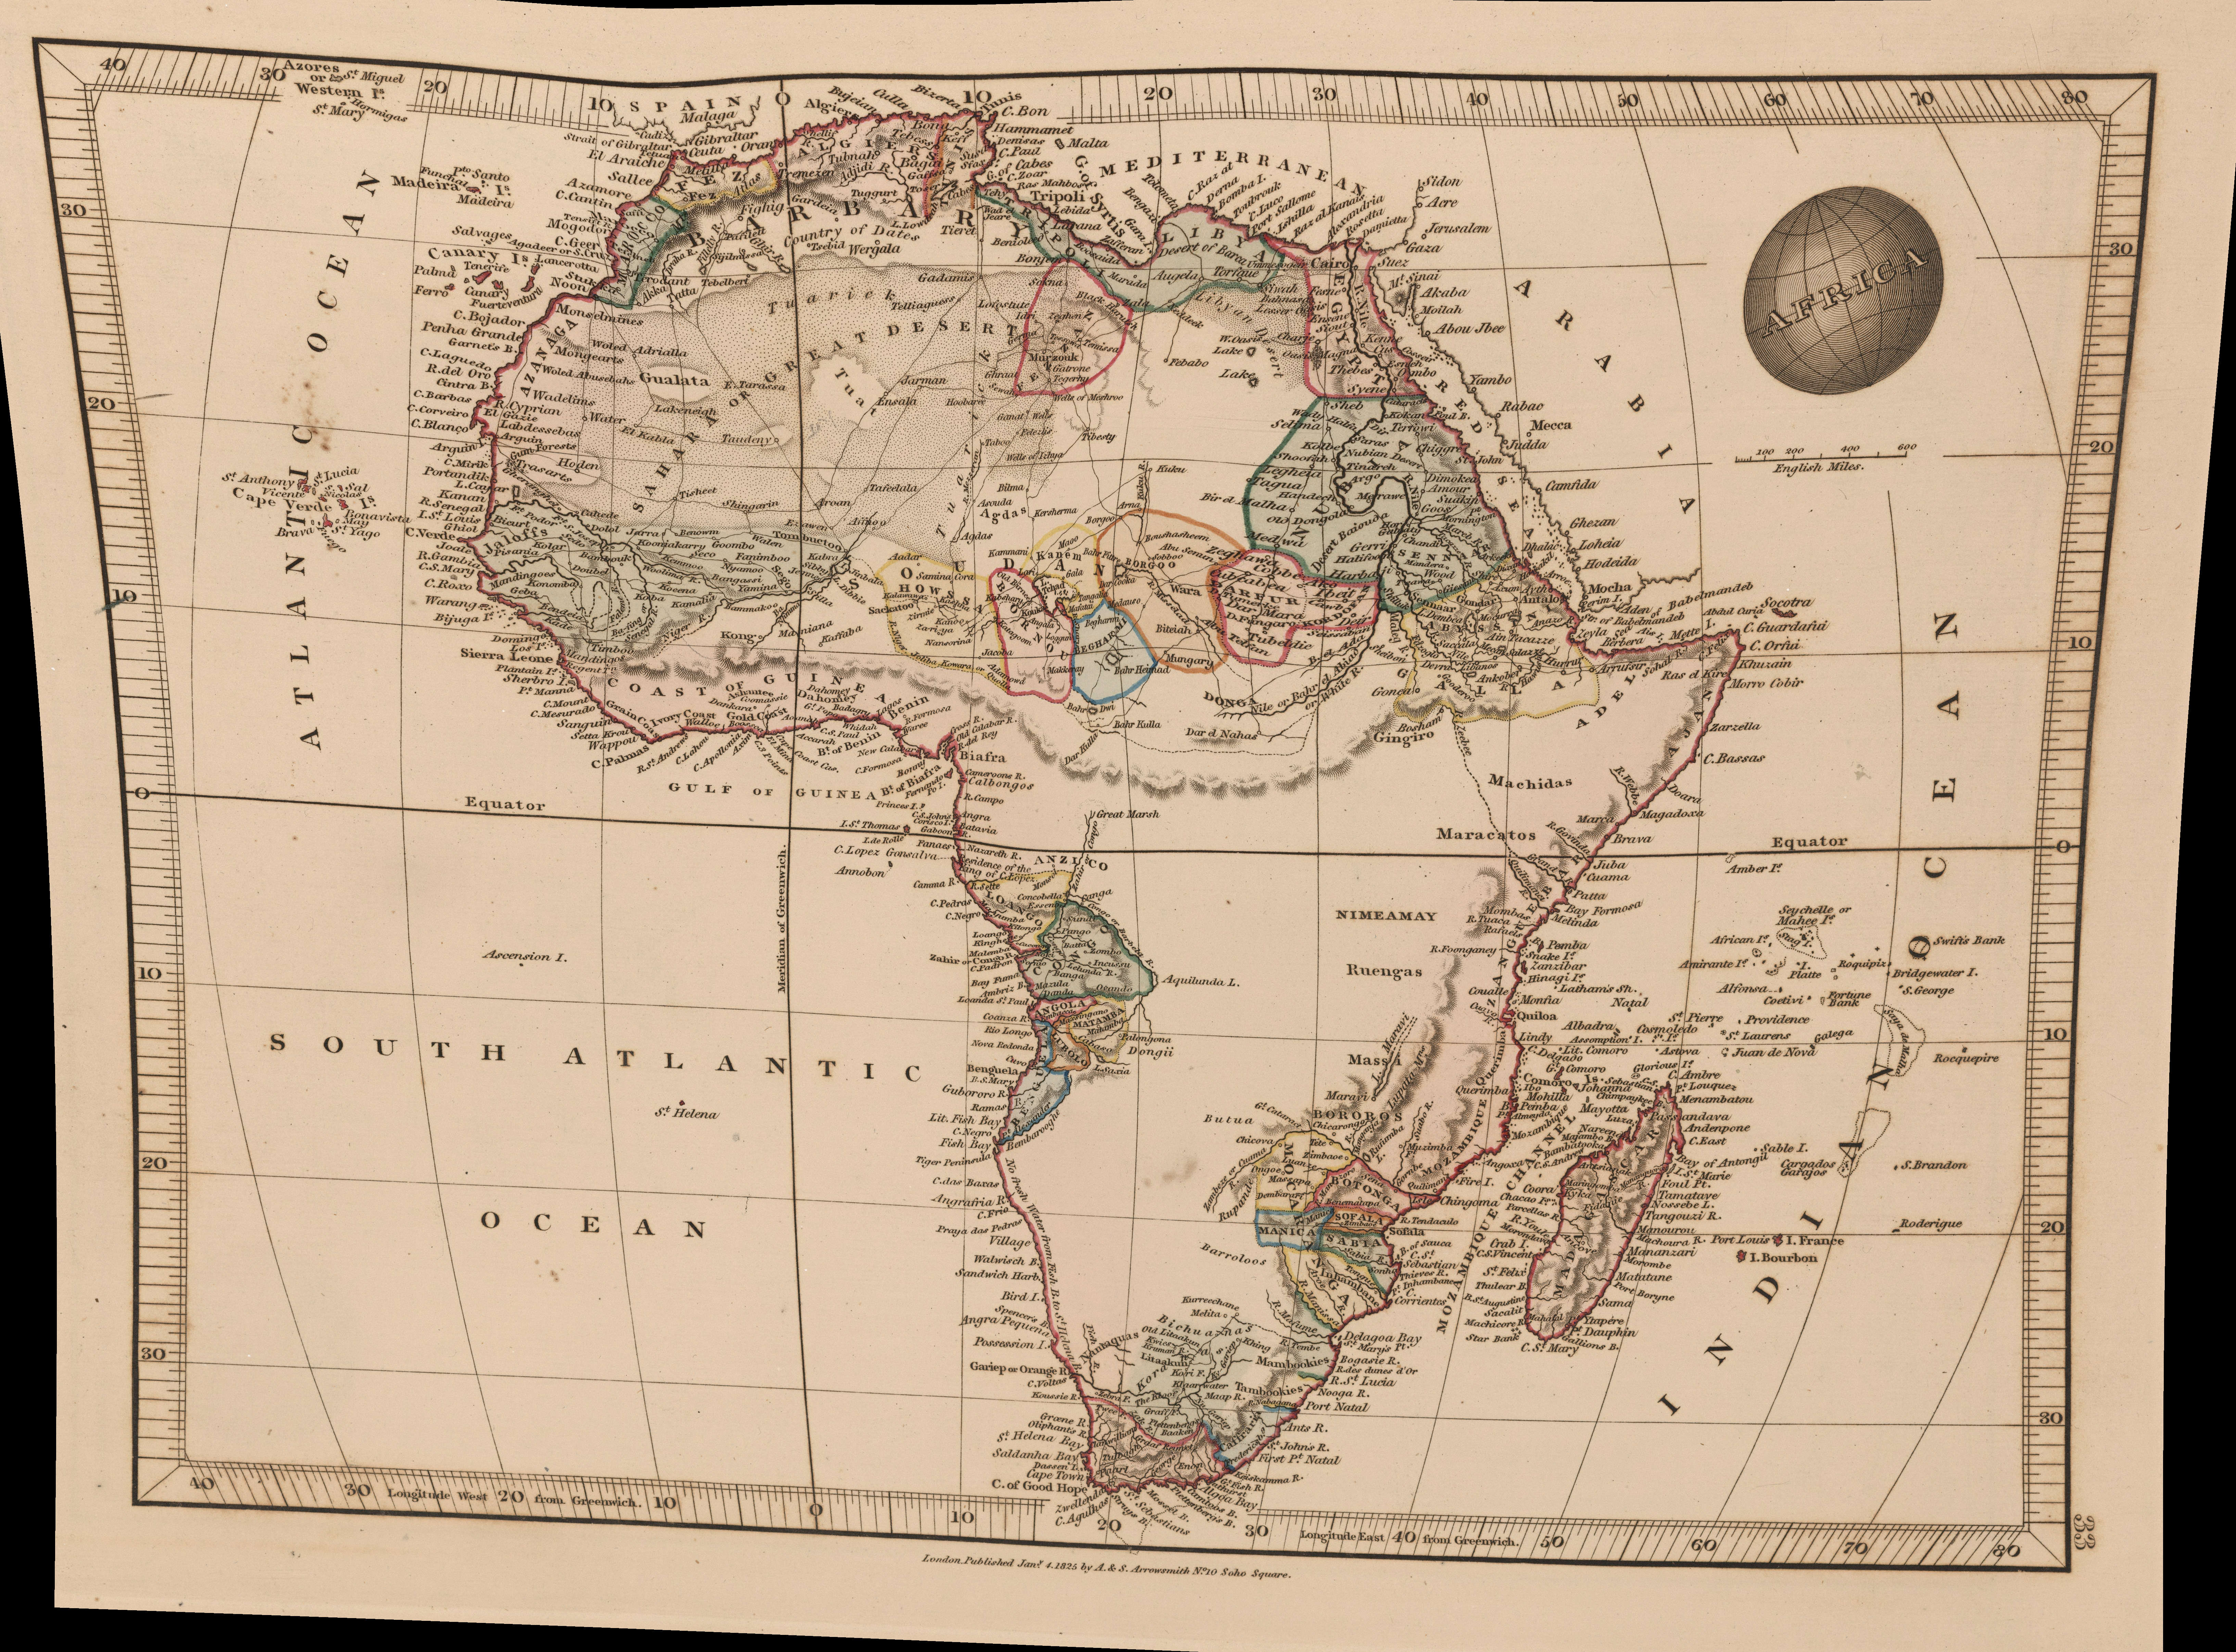
\includegraphics[width=0.8\linewidth]{img/Arrowsmith.jpg}
	\caption{Example of georeferenced map}%
	\label{Arrowsmith}
\end{figure}

%\begin{multicols}{2}

\subsection{The mountains of Kong}

The accuracy of the historical maps used to create the polygons of the Geo-ISD
is a natural concern. Who typically drew these maps? Based on what sources? For
what purposes? And with what level of technical accuracy? 

By tracing the creation of a selection of the maps, I found that most of the
maps from the David Rumsey project are from atlases published for commercial
purposes by individuals or small publishing companies specialized in this type
of publications. Most are from English or American atlases, but French, Italian,
German and other sources are included as well. The maps were based on a
combination of existing maps updated with ``the latest sources" (something
frequently boasted in the title of the atlas), which for the majority of the
period meant explorers/geographers on missions from their respective
geographical societies.\footnote{Later maps additionally draw on the work of
	military surveyors, but as far as I have been able to tell the majority
is still based primarily on the work of explorers and past maps.} In the words
of \citet[47-48]{Stone1995}: `Cartography in Africa [in the 19th century] is
still a mix of measurement, less accurate observations, word of mouth, previous
maps and sources, educated guesses and pure conjecture. Nevertheless a distinct
improvement on the maps of previous periods.'. As a result I expect two types of
bias: bias resulting from measurement errors and bias resulting from
misconceptions (deliberate or not) of what constituted the borders of a polity
at the time. While the quote above might lead one to expect considerable
measurement error, by my estimate this error only amounts to 36.9km on
average.\footnote{Based on the estimated mean distance of the coast in the maps
	to the real coast, along the borders of the states we traced. This
	captures measurement error explicitly, because regardless of where
	states did or did not extend their control, the coast should in the map
	should line up with reality (assuming no reason for the cartographers or
	anyone else to misrepresent the coastline). Indeed, we often used the
	recognizable features along the coast to georeference the maps. This
	means that there are often multiple estimates for each map, reflecting
	how the accuracy is better in some places than in others. If this
	difference was above 100km the maps were deemed too inaccurate and
	excluded from the sample. We did not include error estimates for states
	that lay inland, because consistently matching features from the maps to
real geographical features was not feasible other than when using the coastline,
which provides a visible line of comparison.} Although I have not been able to
find any sources discussing specifically how cartographers determined the
borders of different polities, my best guess it that it in large part relied on
local verbal sources (word of mouth). Both their sources as well as the
cartographers themselves could have induced bias to the resulting maps. At the
very least there should be heterogeneity in the conceptualization of
territoriality. What determines where a given source (or the cartographer in the
second instance) draws the borders of a polity, or how this would vary with
their respective conceptualization of states, polities and ethnic groups, is
impossible do determine. However, thanks to (usually) having multiple maps for
each state, the variation can be leveraged to create a measure of the
\textit{degree} to which a state had a presence in a given area over the time
period as a whole. When maps disagreed on where the various borders were, I
interpret it as either true variation across time, or as an indication of the
ambiguity of where a given state had \emph{de facto} or \emph{de jure} control.
In the areas where all the maps agree we could be quite sure that the given
state entity had real presence.  While in areas where only one map indicated
that the state was presence, this could either be wrong, an indication of
\emph{de jure} as opposed to \emph{de facto} presence or some other form of
limited presence. The coding process of looking at hundreds of maps strengthened
this initial intuition, and the resulting figures of state presence drawn from
the complete data lends it further credence. Most maps should agree
on the core areas of a state while the further away from the core fewer maps
would consider the area part of the state. We believe this approximates the real
ambiguities surrounding where states governed and where they did not, resulting
in a measure of state presence in a given area. Figure \ref{overlay} is an
overlay of all the map polygons of Libya, Tunisia and Egypt. It demonstrates how
the authority of these states faded into the desert, partially overlap at the
borders, and in the Libyan case, its tenuous hold on the Fezzan region. Although
to a lesser degree, one can also see that Libya as a whole spent fewer years as
an independent state than its neighbours in the region.

%\end{multicols}

\begin{figure}[htpb]
	\centering
	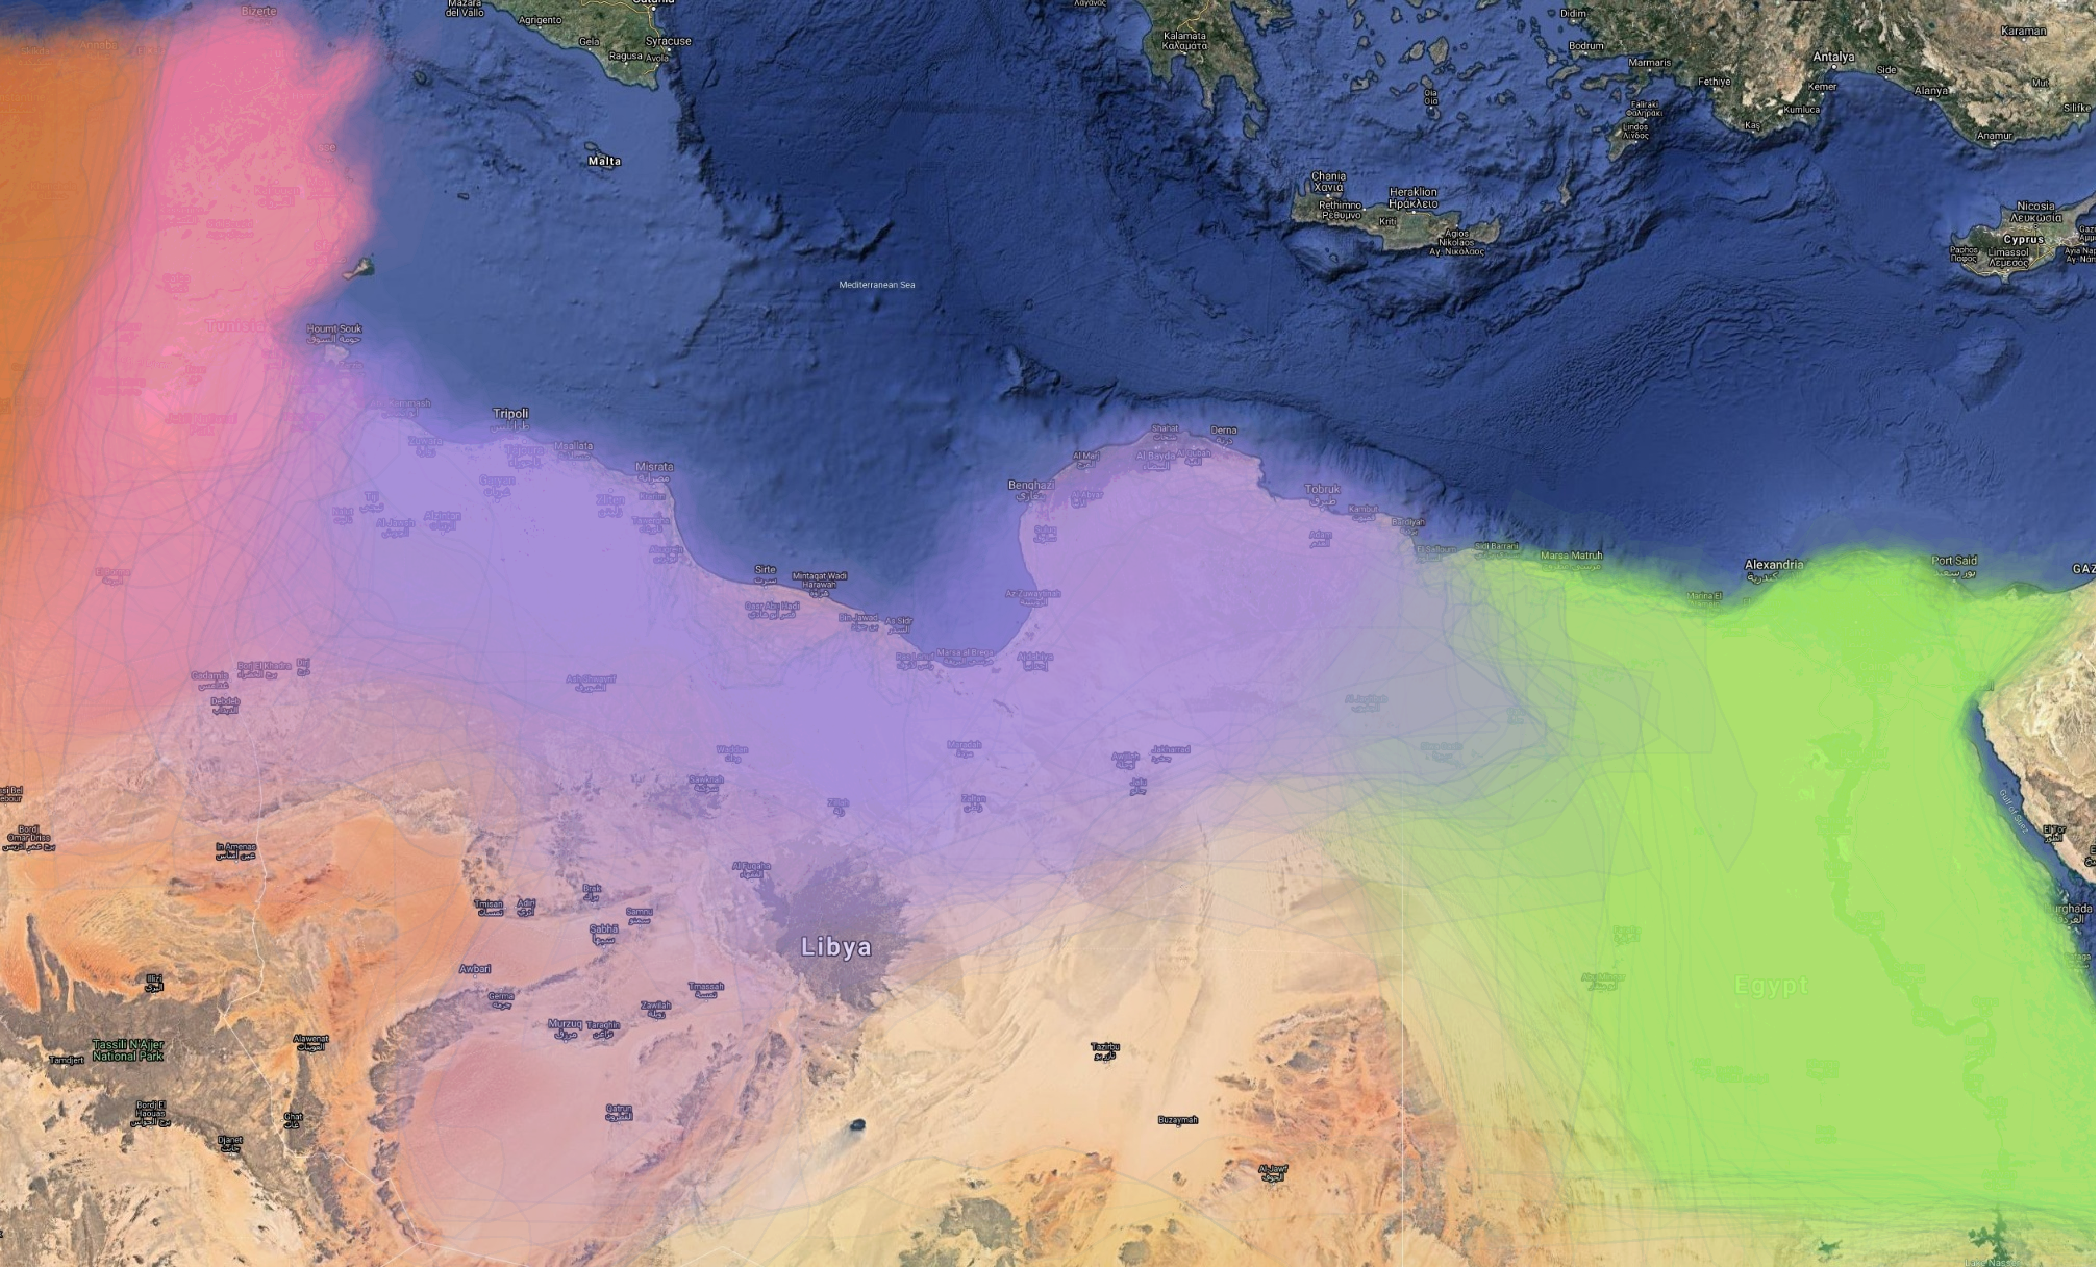
\includegraphics[width=0.8\textwidth,keepaspectratio]{img/TUNLIBEGY.pdf}
	\caption{Overlay of all map polygons of Tunisia, Libya and Egypt}
	\label{overlay}
\end{figure}

%\begin{multicols}{2}

The resulting data can be compiled in different ways, to provide different
insights. Included with the data set are two different measures of
``borderness" (the degree to which an area has historically been on the fringes
of local states), one measuring the overlapping of borders, and one measuring
how many borders pass through an area. For this paper however, I rely on the
measure of `state presence', similar in concept to that of
\citet{Depetris-Chauvin2016}, which was the original purpose for the Geo-ISD.

The data from this project can be aggregated and used in multiple ways and to
produce different variables and measures. All of these indicators are aggregated
over all years for individual PRIO-GRID cells in Africa. The primary indicator
used in this paper is a measure of the presence over time. It is measured by the
number of maps that indicate that a state was present there, counting only those
of the state most often present in that cell. So that if a cell bordering
Tunisia and Libya contains 40 maps of Tunisia and 7 maps of Libya, only the
Tunisian maps are counted. Including the Libyan maps would risk over counting as
it most likely does not represent additional state presence, but rather
overlapping state presence. 

%\end{multicols}

\begin{figure}[htpb]
	\centering
	%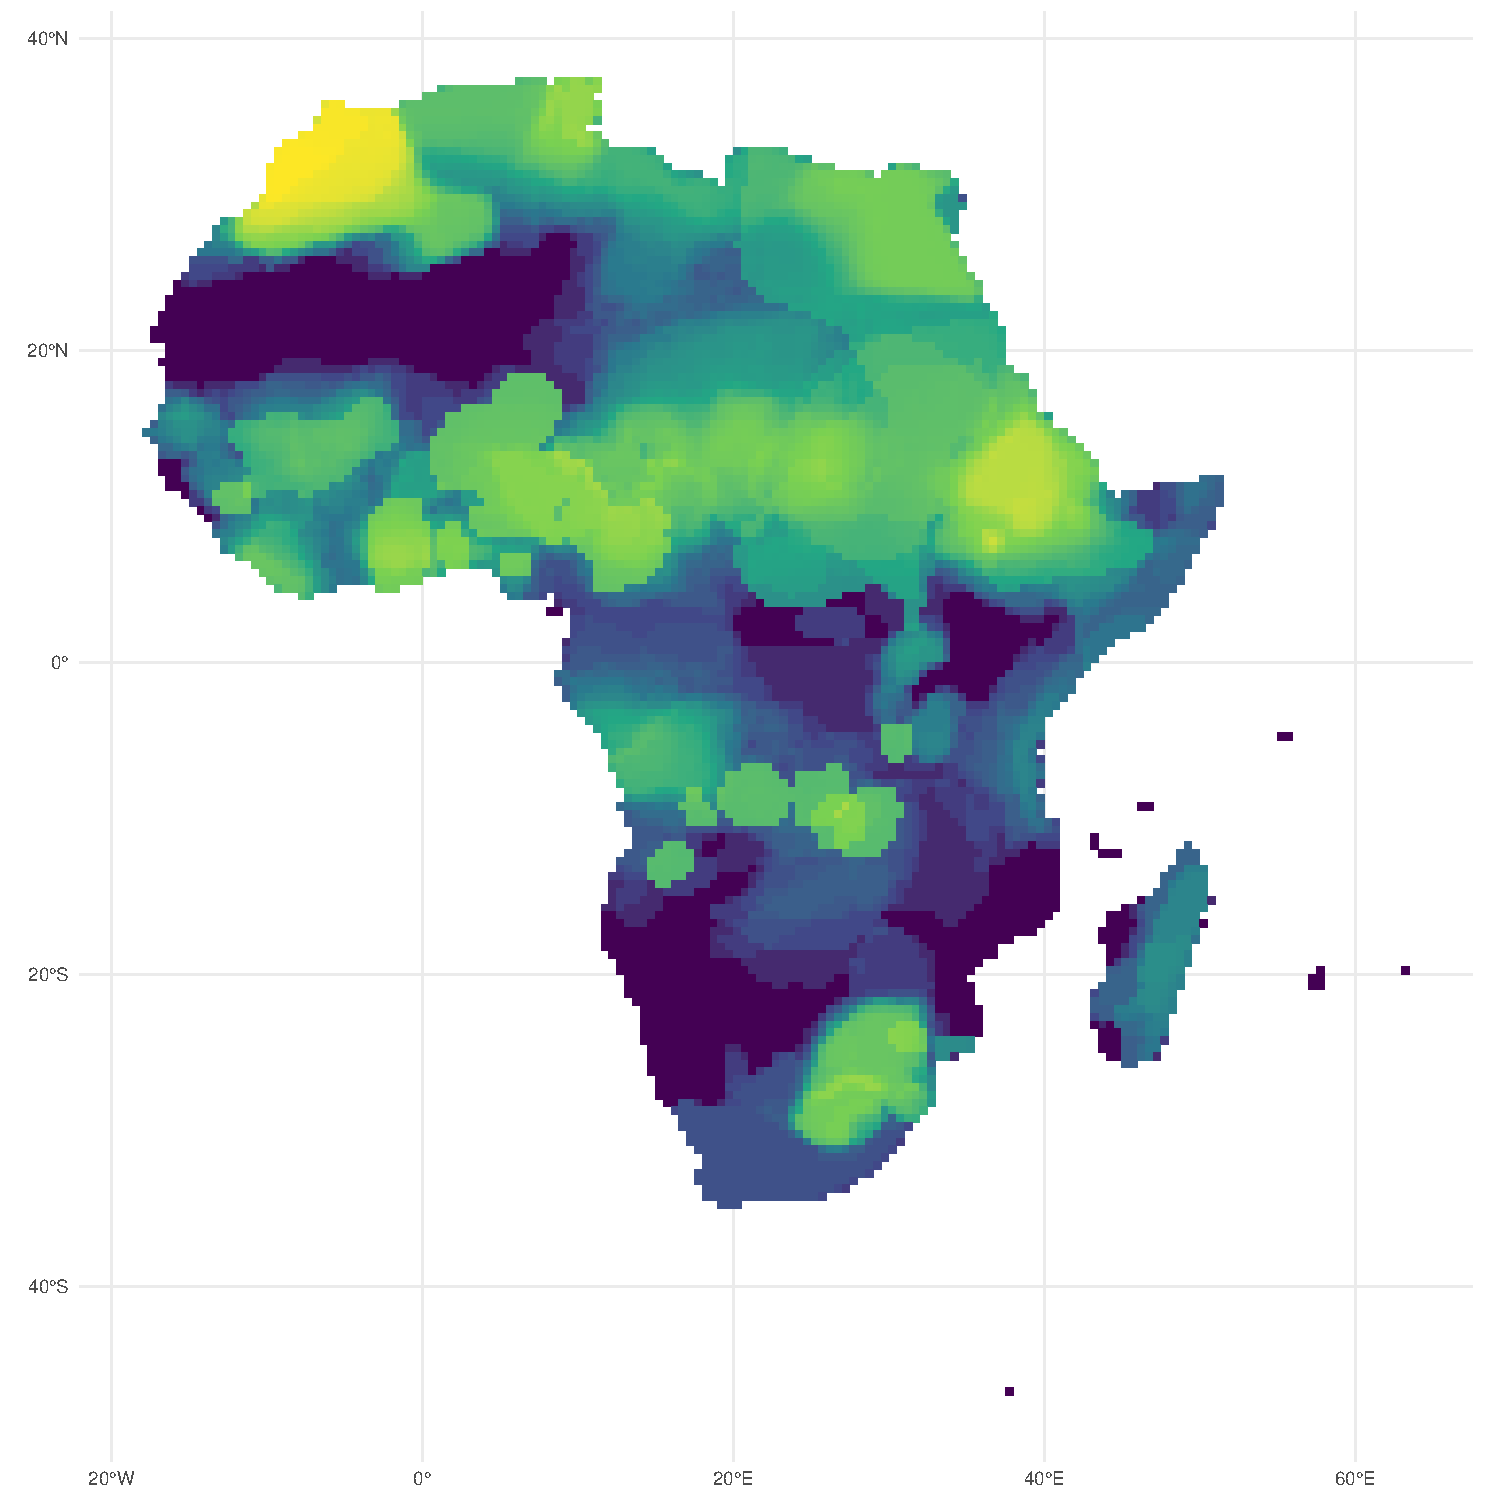
\includegraphics[width=0.8\linewidth]{../Rplot_ln_sp_int.pdf}
	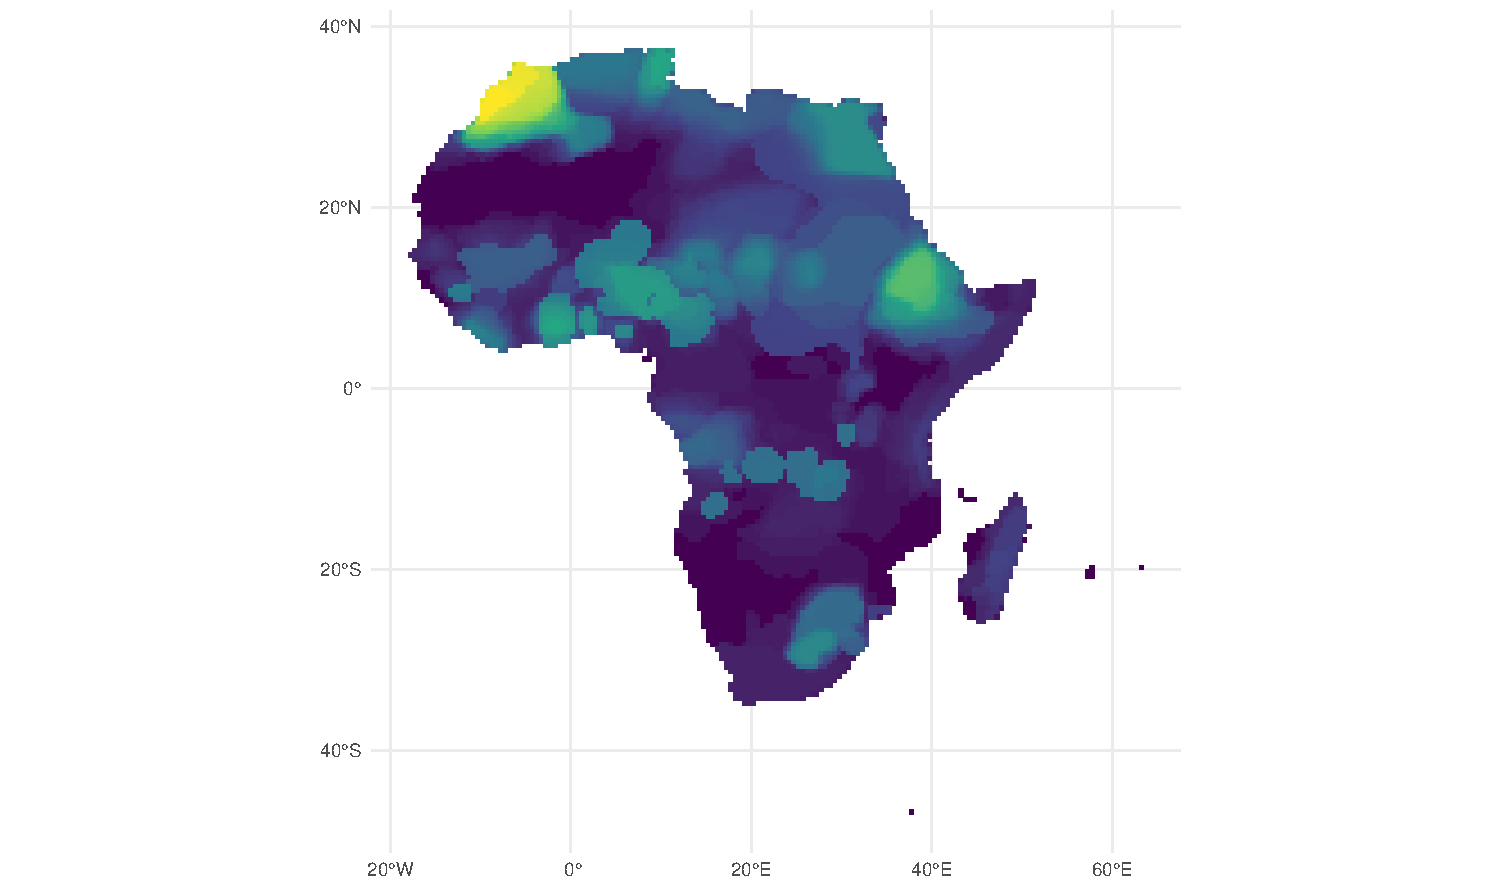
\includegraphics[width=\linewidth]{../R/Output/sqrtSpAll.pdf}
	\caption{State presence (sqrt transformed) with interpolated years based
	on historical atlases.}
	\label{Sp_i}
\end{figure}

\begin{figure}[htpb]
	\centering
	%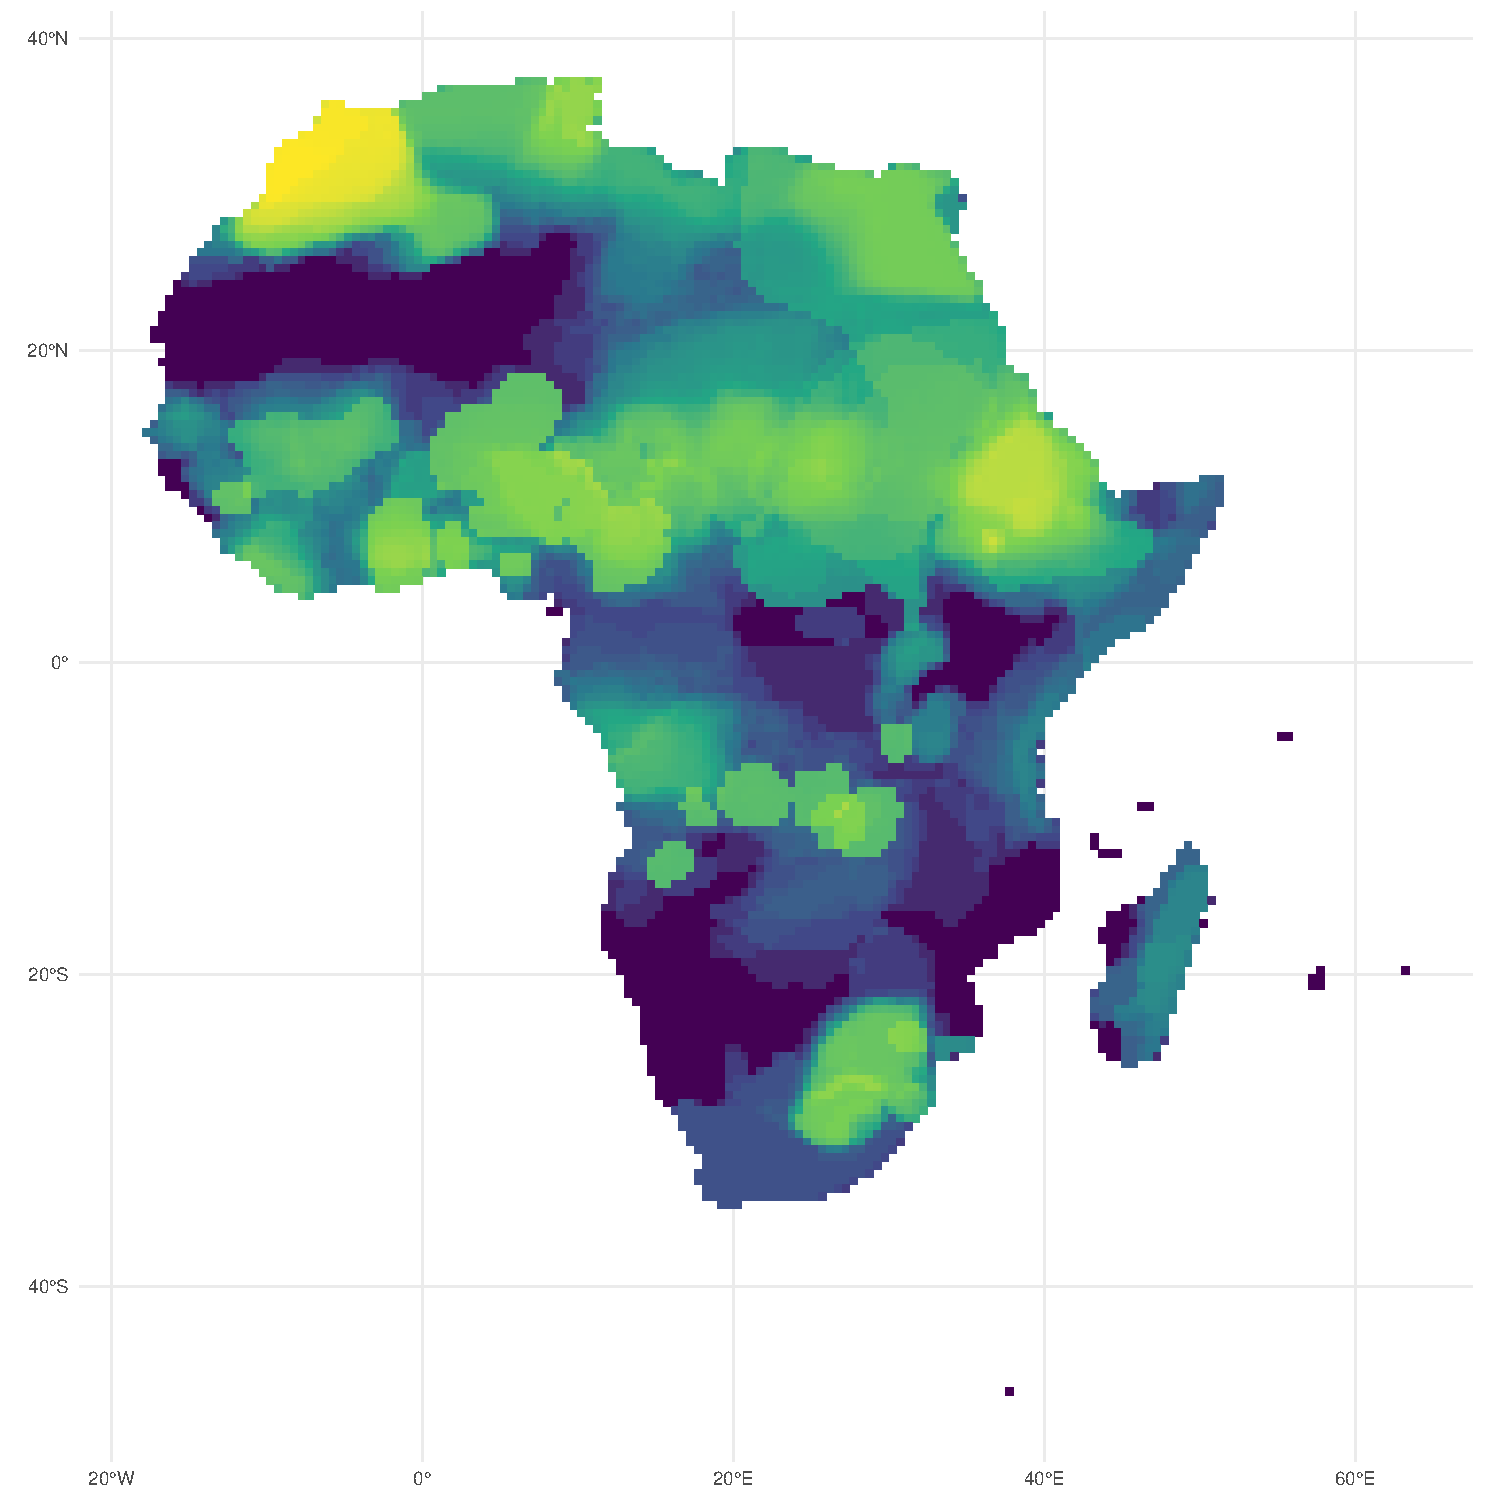
\includegraphics[width=0.8\linewidth]{../Rplot_ln_sp_int.pdf}
	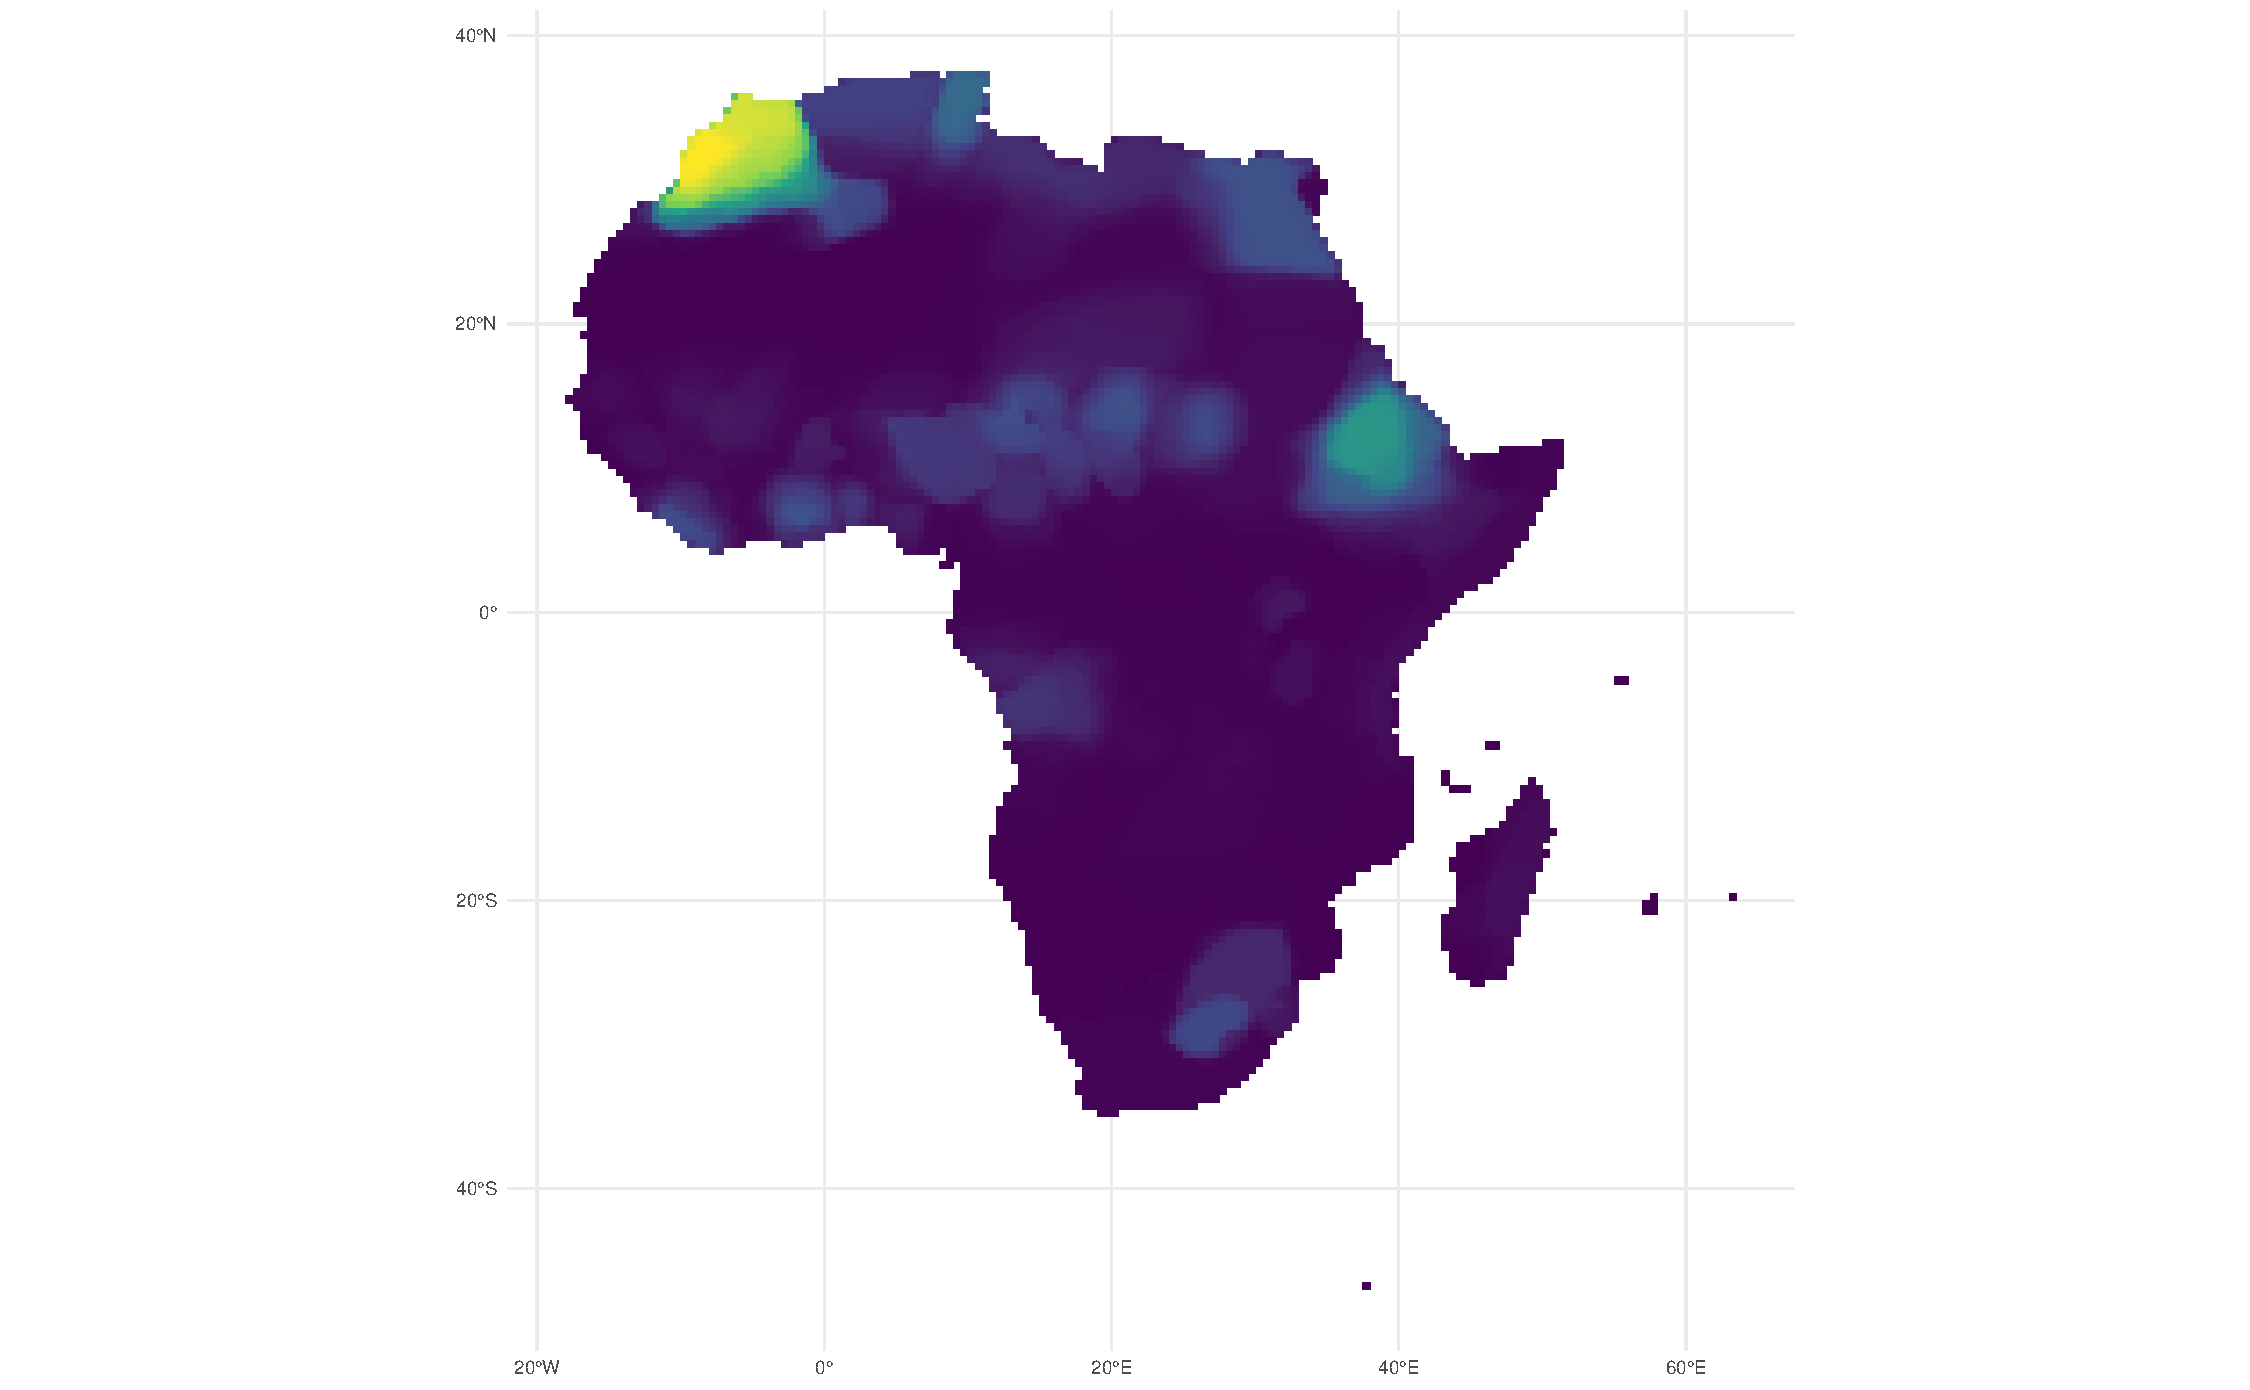
\includegraphics[width=\linewidth]{../R/Output/sp_os_sum.pdf}
	\caption{State presence (sqrt transformed) without interpolated years.}
	\label{Sp}
\end{figure}

%\begin{multicols}{2}

\section{Research design}

\subsection{Dependent variable}

The unit of analysis are PRIO grid cells, which are one degree by one degree
cells \citep{Tollefsen2012}. Due to the explanatory variable being
time-invariant, the analysis is limited to a cross section. Accordingly, the
dependent variables are conflict related fatalities per grid cell in the period
1989-2018 [currently, will update to the latest numbers], excluding events from
conflicts of decolonization. In other words these are cross sectional count
data. The data are from the GED project \citep{Sundberg2013}. I intend for this
to be a general measure of the level of conflict in the post World War 2 period.
While some of the theoretical mechanisms discussed above might be more closely
related to a specific type of state-based conflict, such as wars of secession,
these are difficult to separate entirely. That is, they are unlikely to manifest
\textit{exclusively} as a specific type. This does not mean that the choice of
dependent variable biases in favor or finding a relationship. In fact
\citet{Wishman2021a} finds that pre-colonial state presence has a negative
effect on communal violence events. Fatalities from which are included in the
dependent variable used in the models discussed below.

% Run models excluding org3 fatalities, citing my other paper?
% Would strengthen results but probably not by much. Adds little.

\subsection{Independent variable}

The main explanatory variable is the per grid cell sum of state presence. For
the main model I use measure of state presence from the Geo-ISD that counts all
maps that intersect a given grid cell, even if multiple maps do so in a single
year, but only for the state that has the most presence overall in that grid
cell. This measure has the benefit of including more data, which allows for the
approximation of relative degrees of state presence by one state in any year, as
described in the data section above. At the same time it avoids over counting
state presence where there were overlaps in sovereignty or changes in who
controlled the territory. As a robustness check I also ran models using the
measure that counts if there was any state presence in a grid-cell-year (as a
yearly dummy). In other words, this could be at most 214, and it is more so a
measure of the maximum \textit{extent} of state presence, and is less accurate
in terms of depth. The benefit of this measure is that it avoid the potential
over representation of countries frequently mapped by Europeans, such as the
North African states (proximity) and Darfur (weird obsession?) Again counting
only the presence of the most present state for each grid cell. In both cases
this paper uses the measure which includes interpolated shapes from historical
atlases. Where historical atlases depicted the borders of a state from year x to
y, we created identical shapes for all these years. This has the benefit of
placing a slightly larger emphasis on the historical atlases, at the cost of
being static.\footnote{Equivalent models excluding the interpolated shapes are
included in the Online appendix. Results remain substantially the same for all
specifications.}

Because I do not expect the relationship between pre-colonial state presence to
be linear, and because the data is heavily skewed, the variable is square root
transformed. While log transformation is more commonly used, and does produce a
more evenly distributed variable in this case as well, having to add 1 to
all values could potentially introduce bias [ASK OLE M ABOUT THAT PAPER]. 

\subsection{Controls}

Mountains help in early state formation by providing protection and limiting the
exit options of sedentary farmers \citep{Carneiro1988}. Mountainous terrain has
also been linked with civil conflict by providing shelter for rebel groups
\citep{Hegre2006}, although this relationship is debated 
\citep{Buhaug2002}. The data is from the PRIO-grid data set, but originally 
from \citet{Blyth2002}. 

Water is essential for state formation. States typically formed either as
coastal cities, close to navigable rivers or by the shores of great lakes.
People still tend to live next to a source of water, thus this acts as a proxy
for population density, and fighting usually happens where there are (at least
some) people.  Water could also be related to the conflict measures more
directly by being a non-divisible resource to fight for control over, or
potentially it indicates strategic location, such as river crossings *** SOURCES
NEEDED, evidence is scarce ***. The data on water as a percentage of the grid
surface is from the PRIO-grid data set, but originally from the European Space
Agency \citep{Bontemps2009}.

Distance to coast could affect both state presence and conflict in a number of
ways. First, as state above, states were more likely to be formed along the
coast as it connected cities and people. A special case for Africa is also the
existence of slave raiding/trading states that formed along the eastern and
western coasts of the continent. These states raison d'être was raiding slaves
from tribes and peoples inland and selling them to coastal traders (European in
the West and Arab in the east). \citet{Nunn2008} argues that this state of
affairs left legacies of mistrust and antagonism, which has resulted in
increased levels of current day conflict. Distance to the coast could also be
related to the measure of state presence through the fact that our measure is
based on European observations (maps), which undoubtedly had better coverage
along the coast, especially for the earlier periods. Distance to the coast could
further be related to conflict through lower levels of development. The distance
to coast data is from \citet{Wessel1996}.

As with water, barren terrain could be a (negative) pre-condition for state
building as well as proxy for later population densities, and thus could
correlate with both state presence and levels of conflict. The data is from
\citet{Bontemps2009}.

Almost certainly due to the geographical proximity, and the accompanying
historical familiarity of European map makers to the states of North Africa,
this region is undoubtedly overrepresented in the Geo-ISD data. This affects
Morocco most particularly, as can be clearly seen in figures \ref{Sp_i} and
\ref{Sp}. The reason this affects Morocco in particular is that the remaining
North African states were under Ottoman suzerainty for much of the period.

Population density is only added as an extended control despite the stronger
theoretical expectation that it could be a confounding variable, because there
are no accurate measures of population densities that predate most of the
states in the Geo-ISD. The best available estimates come from the HYDE project
\citep{Goldewijk2016}. In order to predate most of the states in the Geo-ISD I
use the estimates from 1600.

%As a robustness check some models also include measures of temperature (mean and
%variance), precipitation (mean and variance) and forest (remove?), as these have
%been found to affect conflict and could potentially affect state building ***
%Ask Ole Magnus about these, I don't see the connection ***

Distance to borders could be related to state presence because despite their
reputation African borders were not drawn completely at random (or along
meridian lines). For example, the borders of northern Nigeria and Niger were
based on the extent of the Sokoto Caliphate and the neighboring Kanem-Bornu (or
just Bornu) empire \citep{HiribarrenVincent2017AHoB}. Proximity to international
border has also been found to predict conflict \citep{Buhaug2002}. I use the
measure included in the PRIO grid data, which is originally from
\citet{Weidmann2010a}.

\subsection{Alternative measures}

As an alternative to combat related fatalities, I also ran models using the
count of state based conflict events, again excluding the events related to
decolonization. This captures much of the same general level of conflict during
the period as the fatalities measure does, but the focus is slightly different.
Fatalities captures severity of conflict as part of the general conflict level,
whereas the number of conflict events captures the frequency of conflict. This
would be the difference between few, or short, but highly lethal conflicts,
versus long winded conflict of relatively low intensity, or recurring conflicts.
I do not expect there to be a substantial difference in the results from these
measures based on the theory presented above.

In addition to the square root transformed version of the main independent
variable, I also ran models using the more common log transformation as well as
models using a non-transformed variable. For the logged models result remained
substantially the same (see online appendix eventually). Whereas the
non-transformed models while remaining significantly positive, predicted effects
that were substantially meaningless (an increase in pre-colonial state presence
by 10 was still not enough to predict a .01 increase in the number of fatalities
across the whole period).

\subsection{Modelling}

The main models presented below are negative binomial models to account for the
dependent variable being count data (count of deaths (fatalities) and count of
conflict events (state based)). A fitness test for whether negative binomial or
Poisson regression is most appropriate, was conducted and confirmed that
negative binomial produced the best fit.

Because there are a great number of zeroes in the dependent variable, as well
as for theoretical reasons there it is reasonable to assume that there are a
number of excess zeros. Hence, a zero inflated negative binomial is the most
appropriate approach. However, most specifications of the models did not
converge unless all right hand side variable were normalized to around their
mean. This complicates interpretations of substantial effects, but signs and
significance remained unchanged from the main models for all specifications (see
Online appendix eventually).

Because of the size of the grid cells I argue it is safe to assume that events
and fatalities are largely independent across grid cells (that is independent
across space). However, some models were run with queen pattern spatial lags,
most of which did not converge. Those that did successfully converge, remained
substantially similar to the main models.

\section{Preliminary results}

The positive relationship between state presence and conflict is robust across
all models. The results of the interaction models might help explain the
relationship. As seen in Figure \ref{deaths_int}, state presence is negatively
correlated with both conflict measure close to the capital, but becomes positive
and significant further away from the capital. This supports an interpretation
that state presence can be conflict reducing in those cases where it makes a
country less artificial for all the reasons outlined by the conflict reducing
arguments in the literature. Taken together however, the results indicate that
the negative effects of higher values of state presence further away from the
capitals of Africa outweighs these conflict reducing effects. 

%\end{multicols}

%\begin{figure}[htpb]
%	\centering
%	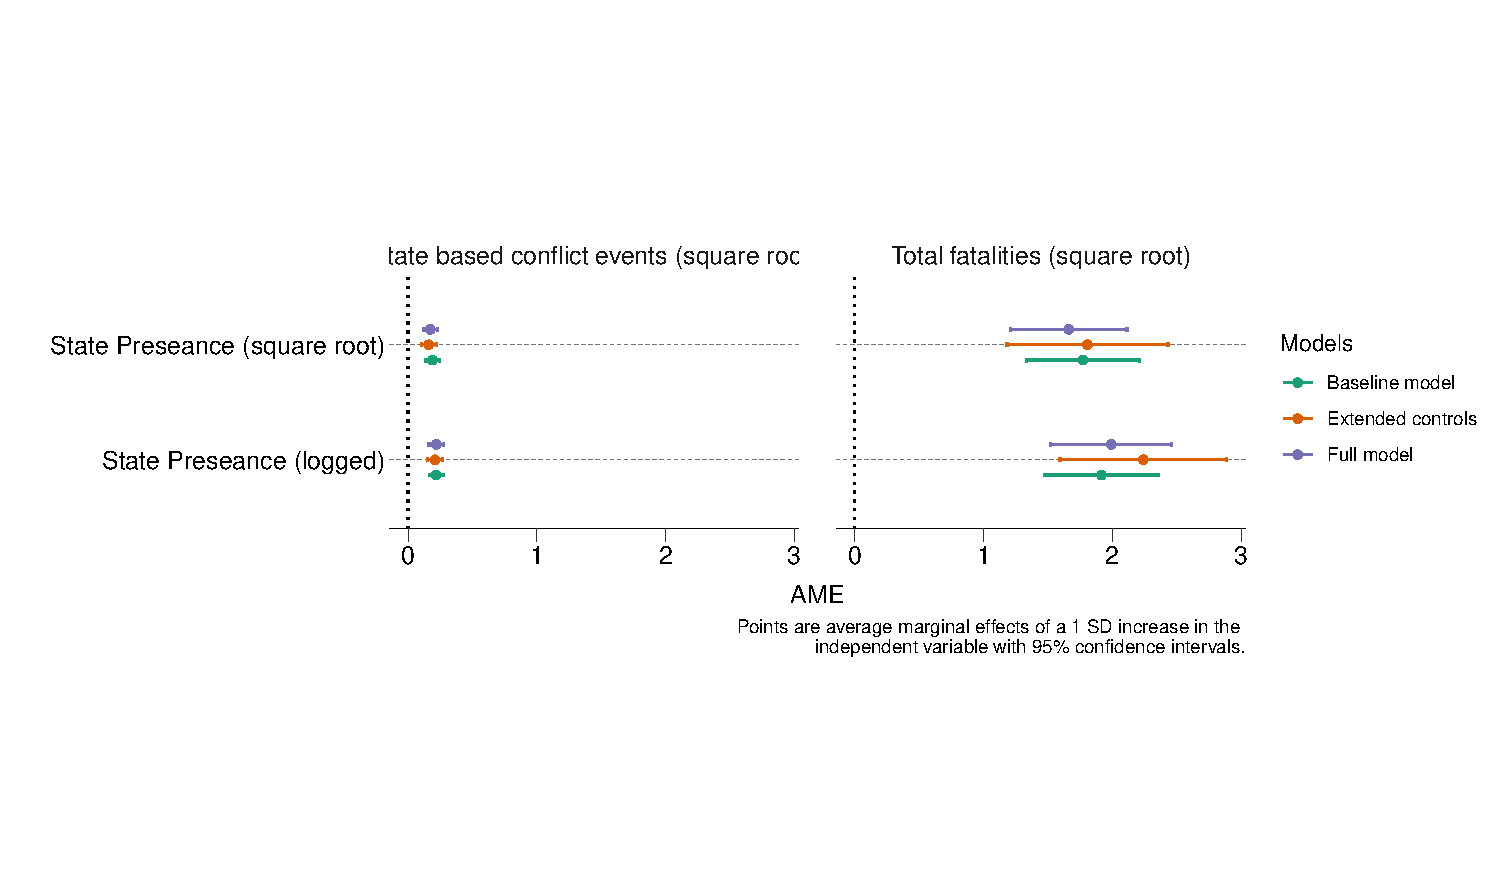
\includegraphics[width=\linewidth]{"../R/Output/conflictMargins.pdf"}
%	\caption{}
%	\label{margins}
%\end{figure}

\begin{figure}[htpb]
	\centering
	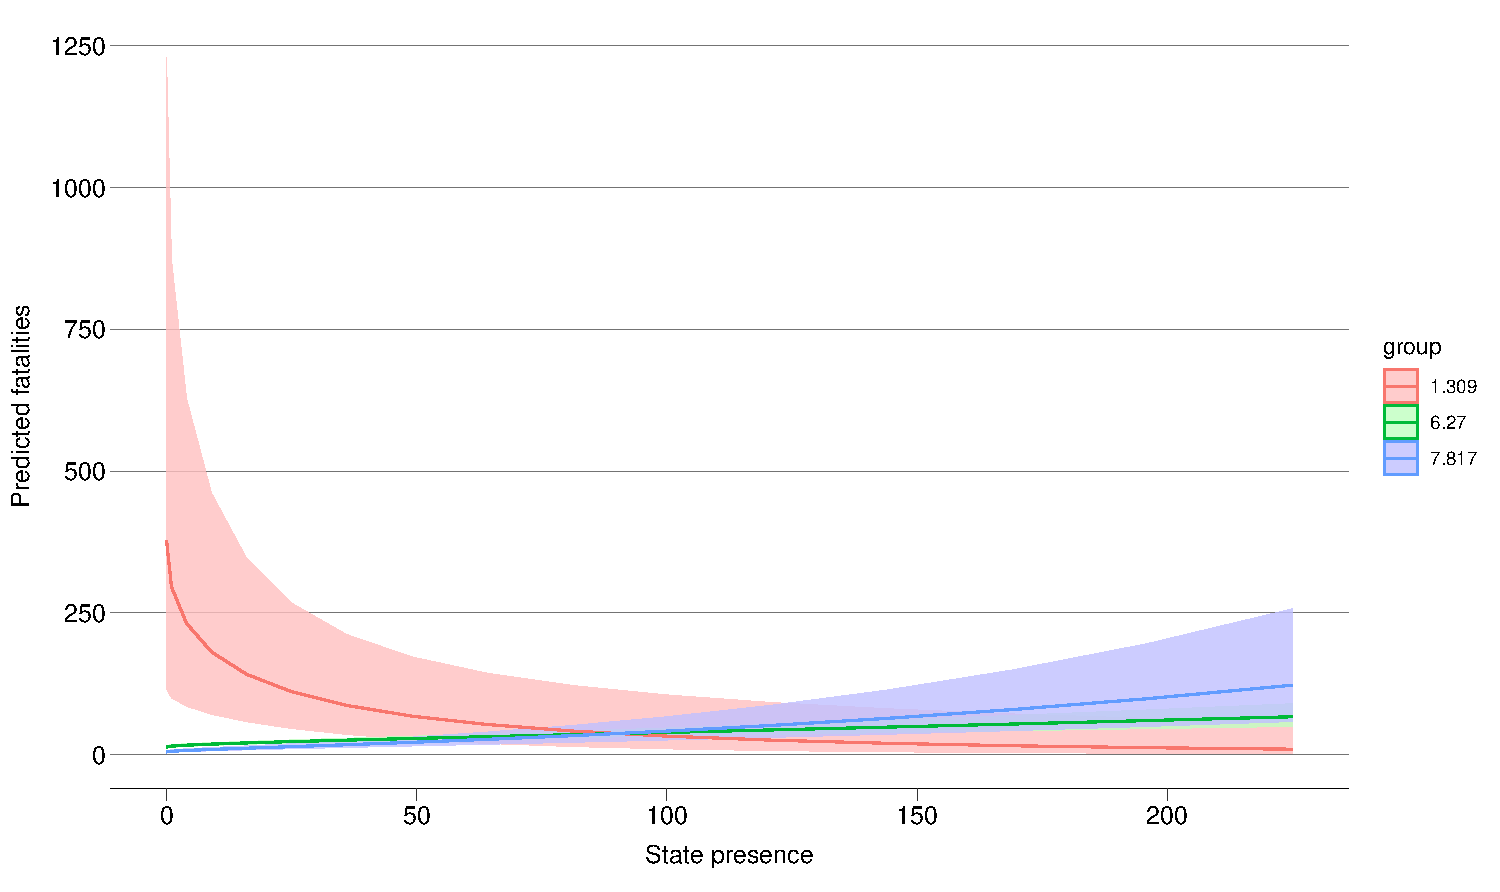
\includegraphics[width=\linewidth]{"../R/Output/deathsIntPlot.pdf"}
	\caption{}
	\label{deaths_int}
\end{figure}

%\begin{figure}[htpb]
%	\centering
%	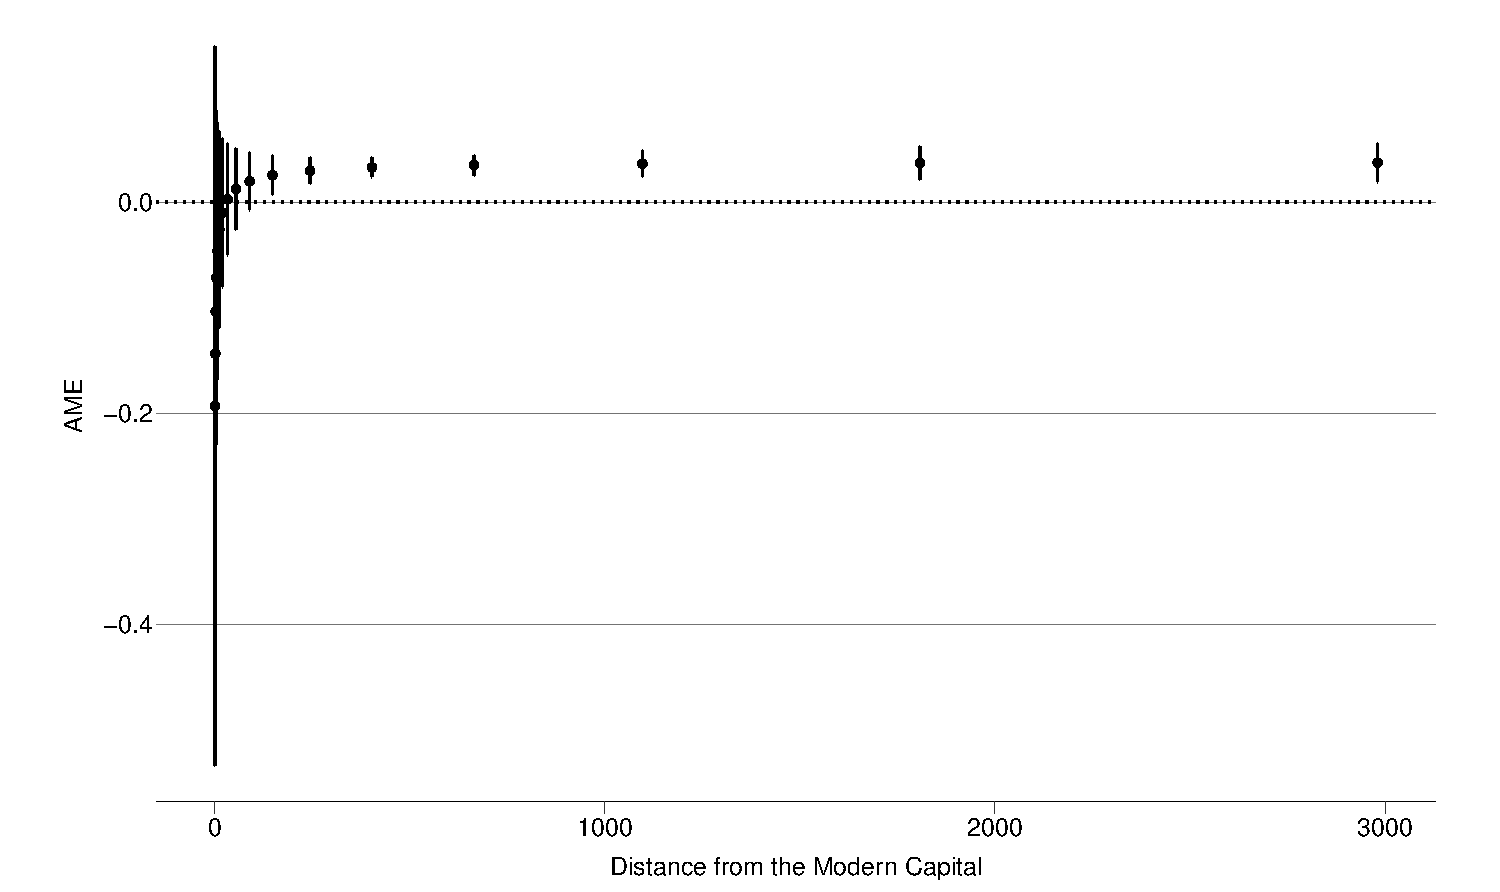
\includegraphics[width=\linewidth]{"../R/Output/state_based_int_plot.pdf"}
%	\caption{}
%	\label{sb_int}
%\end{figure}

%\begin{multicols}{2}

\section{Conclusion}

Although effects are substantially small, they are robust, and indicate that
pre-colonial states have played some role in shaping modern levels of conflict.
Crucially, the interaction models show that previous assumptions about both
conflict inducing and conflict reducing effects of pre-colonial statehood are
not necessarily in contention. In areas where the remnants of prior statehood,
be they traditions, institutions of social networks, form a continuum to the
modern state, they could well help states govern more peacefully. On the other
hand, when placed in opposition to a central government such remnants seems to
increase the level conflict.

%\end{multicols}

\pagebreak

\bibliographystyle{agsm}
\bibliography{../lib.bib}

\pagebreak
\section*{Appendix}


\begin{sidewaystable}
\begin{center}
\scalebox{1}{
\begin{tabular}{l c c c c c c}
\hline
 & Baseline & Extended Controls & Baseline & Extended Controls & Baseline & Extended Controls \\
\hline
(Intercept)     & $3.26^{***}$  & $2.29^{***}$  & $3.65^{***}$  & $2.63^{***}$  & $4.07^{***}$  & $2.95^{***}$  \\
                & $(0.13)$      & $(0.14)$      & $(0.12)$      & $(0.13)$      & $(0.11)$      & $(0.13)$      \\
logSpAll        & $0.30^{***}$  & $0.28^{***}$  &               &               &               &               \\
                & $(0.03)$      & $(0.03)$      &               &               &               &               \\
mountains\_mean & $2.36^{***}$  & $1.24^{***}$  & $2.29^{***}$  & $1.08^{***}$  & $2.21^{***}$  & $1.09^{***}$  \\
                & $(0.19)$      & $(0.19)$      & $(0.19)$      & $(0.19)$      & $(0.20)$      & $(0.19)$      \\
water\_gc       & $0.02^{***}$  & $0.01^{***}$  & $0.03^{***}$  & $0.01^{***}$  & $0.02^{***}$  & $0.01^{***}$  \\
                & $(0.00)$      & $(0.00)$      & $(0.00)$      & $(0.00)$      & $(0.00)$      & $(0.00)$      \\
barren\_gc      & $-0.03^{***}$ & $-0.02^{***}$ & $-0.03^{***}$ & $-0.02^{***}$ & $-0.03^{***}$ & $-0.02^{***}$ \\
                & $(0.00)$      & $(0.00)$      & $(0.00)$      & $(0.00)$      & $(0.00)$      & $(0.00)$      \\
distcoast       & $0.00^{***}$  & $0.00^{***}$  & $0.00^{***}$  & $0.00^{***}$  & $0.00^{***}$  & $0.00^{***}$  \\
                & $(0.00)$      & $(0.00)$      & $(0.00)$      & $(0.00)$      & $(0.00)$      & $(0.00)$      \\
logPopd         &               & $1.03^{***}$  &               & $1.03^{***}$  &               & $1.05^{***}$  \\
                &               & $(0.07)$      &               & $(0.07)$      &               & $(0.07)$      \\
bdist3          &               & $-0.00^{*}$   &               & $-0.00^{*}$   &               & $-0.00^{*}$   \\
                &               & $(0.00)$      &               & $(0.00)$      &               & $(0.00)$      \\
sqrtSpAll       &               &               & $0.10^{***}$  & $0.09^{***}$  &               &               \\
                &               &               & $(0.01)$      & $(0.01)$      &               &               \\
SpAll10         &               &               &               &               & $0.00^{***}$  & $0.00^{***}$  \\
                &               &               &               &               & $(0.00)$      & $(0.00)$      \\
\hline
AIC             & $43066.10$    & $42817.43$    & $43101.68$    & $42851.53$    & $43143.35$    & $42890.13$    \\
BIC             & $43116.91$    & $42882.75$    & $43152.48$    & $42916.85$    & $43194.16$    & $42955.45$    \\
Log Likelihood  & $-21526.05$   & $-21399.71$   & $-21543.84$   & $-21416.77$   & $-21564.67$   & $-21436.07$   \\
Deviance        & $5340.87$     & $5355.31$     & $5338.89$     & $5353.37$     & $5336.65$     & $5351.13$     \\
Num. obs.       & $10492$       & $10482$       & $10492$       & $10482$       & $10492$       & $10482$       \\
\hline
\multicolumn{7}{l}{\scriptsize{$^{***}p<0.001$; $^{**}p<0.01$; $^{*}p<0.05$; $^{\cdot}p<0.1$}}
\end{tabular}
}
\caption{Fatalities}
\label{deaths}
\end{center}
\end{sidewaystable}

%
\begin{sidewaystable}
\begin{center}
\scalebox{1}{
\begin{tabular}{l c c c c}
\toprule
 & Geography & North Africa & Population densisty & Distance
		  to border \\
\midrule
Precolonial state presence (sqrt)        & $0.07^{***}$  & $0.05^{***}$  & $0.04^{***}$  & $0.04^{***}$    \\
                                         & $(0.01)$      & $(0.01)$      & $(0.01)$      & $(0.01)$        \\
Precolonial state presence (sqrt)        & $0.07^{***}$  & $0.05^{***}$  & $0.04^{***}$  & $0.04^{***}$    \\
                                         & $(0.01)$      & $(0.01)$      & $(0.01)$      & $(0.01)$        \\
Mountainous terrain                      & $0.87^{***}$  & $0.81^{***}$  & $-0.22$       & $-0.28^{\cdot}$ \\
                                         & $(0.16)$      & $(0.16)$      & $(0.15)$      & $(0.15)$        \\
Water (\%)                               & $-0.01^{*}$   & $-0.01^{*}$   & $-0.01^{**}$  & $-0.01^{***}$   \\
                                         & $(0.00)$      & $(0.00)$      & $(0.00)$      & $(0.00)$        \\
Barren (\%)                              & $-0.02^{***}$ & $-0.02^{***}$ & $-0.01^{***}$ & $-0.01^{***}$   \\
                                         & $(0.00)$      & $(0.00)$      & $(0.00)$      & $(0.00)$        \\
Distance to coast (log)                  & $-0.16^{***}$ & $-0.14^{***}$ & $-0.11^{***}$ & $-0.08^{***}$   \\
                                         & $(0.02)$      & $(0.02)$      & $(0.02)$      & $(0.02)$        \\
Population density (log)                 &               &               & $1.00^{***}$  & $0.94^{***}$    \\
                                         &               &               & $(0.06)$      & $(0.06)$        \\
Distance to international boundary (log) &               &               &               & $-0.20^{***}$   \\
                                         &               &               &               & $(0.04)$        \\
North Africa                             &               & $0.51^{***}$  & $0.38^{**}$   & $0.47^{***}$    \\
                                         &               & $(0.13)$      & $(0.12)$      & $(0.12)$        \\
\midrule
AIC                                      & $20314.22$    & $20297.34$    & $20007.10$    & $19979.16$      \\
BIC                                      & $20364.33$    & $20354.61$    & $20071.52$    & $20050.74$      \\
Log Likelihood                           & $-10150.11$   & $-10140.67$   & $-9994.55$    & $-9979.58$      \\
Deviance                                 & $4106.74$     & $4112.96$     & $4158.66$     & $4164.26$       \\
Num. obs.                                & $9492$        & $9492$        & $9492$        & $9492$          \\
\bottomrule
\multicolumn{5}{l}{\scriptsize{$^{***}p<0.001$; $^{**}p<0.01$; $^{*}p<0.05$; $^{\cdot}p<0.1$}}
\end{tabular}
}
\caption{State based conflict events}
\label{state_based}
\end{center}
\end{sidewaystable}


\begin{sidewaystable}
\begin{center}
\scalebox{1}{
\begin{tabular}{l c c}
\hline
 & Baseline & Extended Controls \\
\hline
(Intercept)          & $7.59^{***}$  & $5.66^{***}$  \\
                     & $(0.60)$      & $(0.60)$      \\
sqrtSpAll            & $-0.18^{*}$   & $-0.40^{***}$ \\
                     & $(0.08)$      & $(0.08)$      \\
logCapdist           & $-0.69^{***}$ & $-0.50^{***}$ \\
                     & $(0.10)$      & $(0.10)$      \\
mountains\_mean      & $2.00^{***}$  & $1.14^{***}$  \\
                     & $(0.19)$      & $(0.19)$      \\
water\_gc            & $0.02^{***}$  & $0.01^{***}$  \\
                     & $(0.00)$      & $(0.00)$      \\
barren\_gc           & $-0.03^{***}$ & $-0.02^{***}$ \\
                     & $(0.00)$      & $(0.00)$      \\
distcoast            & $0.00^{***}$  & $0.00^{***}$  \\
                     & $(0.00)$      & $(0.00)$      \\
sqrtSpAll:logCapdist & $0.04^{***}$  & $0.08^{***}$  \\
                     & $(0.01)$      & $(0.01)$      \\
logPopd              &               & $1.06^{***}$  \\
                     &               & $(0.08)$      \\
bdist3               &               & $-0.00^{*}$   \\
                     &               & $(0.00)$      \\
\hline
AIC                  & $43018.78$    & $42824.88$    \\
BIC                  & $43084.10$    & $42904.71$    \\
Log Likelihood       & $-21500.39$   & $-21401.44$   \\
Deviance             & $5343.75$     & $5355.14$     \\
Num. obs.            & $10492$       & $10482$       \\
\hline
\multicolumn{3}{l}{\scriptsize{$^{***}p<0.001$; $^{**}p<0.01$; $^{*}p<0.05$; $^{\cdot}p<0.1$}}
\end{tabular}
}
\caption{Fatalities * Distance to capital}
\label{interaction_deaths}
\end{center}
\end{sidewaystable}


\end{document}


